% Compile with:
% latexmk -pdf -pvc -interaction=nonstopmode
%\documentclass[aspectratio=169,draft]{beamer}
\documentclass[aspectratio=169]{beamer}
\usetheme{UniBern}

\title{X-ray microtomography}
\author{David Haberthür}
\date{December 20, 2019 | \href{https://ilias.unibe.ch/ilias.php?ref_id=1555744&cmd=infoScreen&cmdClass=ilrepositorygui&cmdNode=y2&baseClass=ilrepositorygui}{9256-HS2019-0: Advanced Microscopy}}

%\includeonlyframes{current}
%then....
%\begin{frame}[label=current]
%\end{frame}

\usepackage[backend=biber,
	style=numeric,
	url=false,
	isbn=true,
	maxnames=1,
	sorting=none]{biblatex}
	\addbibresource{../../../Documents/library.bib}
\usepackage{standalone}
\usepackage{tikz}
	\usetikzlibrary{spy}
	%\usetikzlibrary{external}
	%\tikzexternalize[prefix=tikz-externals/] % externalize tikz figures into pdf frames, speeds up compilation
	\tikzset{shadowed/.style={preaction={transform canvas={shift={(1pt,-1pt)}},draw=ubRed}}}
\usepackage{shadowtext}  % for the shadowed scalebar
	\shadowoffset{1pt}
	\shadowcolor{ubRed}
\usepackage{pgfplots}
	\pgfplotsset{compat=newest}
\usepackage[detect-all=true,
	range-phrase=--,
	range-units=single,
	binary-units=true,
	per-mode=symbol,
	per-symbol=/]{siunitx}
\usepackage{microtype}
\usepackage[absolute,overlay]{textpos} %for the \source{} command
\usepackage[missing=master]{gitinfo2} % GitHub Actions don't pull in the commit hash, so we just show `Master'
\usepackage{xspace}
\usepackage{ccicons}
\usepackage[version=4]{mhchem}
\usepackage{animate}
\usepackage{fontawesome5}
\usepackage{csquotes}
\usepackage{listings}
	\lstset{frame=single,
		%backgroundcolor = \color{lightgray},
		basicstyle=\tiny\ttfamily
		}
\usepackage{pgfplotstable}
\usepackage{booktabs}
\usepackage{colortbl}
\usepackage{lipsum} %for alignment testing

% Some often used abbreviations/commands
\newcommand{\everyframe}{1} % use only every nth frame for the animations
\newcommand{\imwidth}{\linewidth}% set global image width
\newcommand{\imheight}{0.618\paperheight}% set global image height
\newlength\imagewidth% needed for scalebars
\newlength\imagescale% needed for scalebars
\newcommand{\uct}{\si{\micro}CT\xspace}% make our life easier
\newcommand{\eg}{e.\,g.\xspace}%
\newcommand{\ie}{i.\,e.\xspace}%

% Define complementary colors to ubRed
\definecolor{ubRedComplementary1}{HTML}{00a1e6}
\definecolor{ubRedComplementary2}{HTML}{00e645}

% change tikz font to slide font
% https://tex.stackexchange.com/a/33329/828
\usepackage[eulergreek]{sansmath}
	\pgfplotsset{tick label style = {font=\sansmath\sffamily},
		every axis label = {font=\sansmath\sffamily},
		legend style = {font=\sansmath\sffamily},
		label style = {font=\sansmath\sffamily}
		}

% Globally thicker lines in with tikz
% https://tex.stackexchange.com/a/206769/828
\tikzset{every picture/.style={thick}}

% And thicker plots by default
% https://tex.stackexchange.com/a/235439/828
% https://tex.stackexchange.com/q/262486/828
\pgfplotsset{%
	every axis plot/.append style={thick},
	every axis/.append style={thick}
	every axis plot post/.append style={every mark/.append style={thick}}
	}

% stripped-down plot styling
% Based on https://tex.stackexchange.com/a/155210/828
% And then start each plot with `\begin{axis}[tuftelike,'
\pgfkeys{%
	/pgfplots/simplified/.style={%
		tick style={major tick length=0pt},
%		separate axis lines,
%		axis x line*=bottom,
%		axis x line shift=10pt,
%		xlabel shift=1pt,
%		axis y line*=left,
%		axis y line shift=10pt,
		ymajorgrids=true,
		axis line style={draw=none},
%		ylabel shift=1pt
		}
	}

% Acknowledge images just below them
% Based on https://tex.stackexchange.com/a/282637/828
\newcommand{\source}[2]{%
	% Print out (short) link under image, with small text
	\raisebox{-1.618ex}{%
		\makebox[0pt][r]{%
			\scriptsize\href{http://#1}{#1} #2%
			}%
		}%
	}%
\newcommand{\sourcecite}[2]{%
	% Cite (an image from) a reference
	\raisebox{-1.618ex}{%
		\makebox[0pt][r]{%
			\scriptsize From \cite{#1}, #2%
			}%
		}%
	}%
\newcommand{\sourcelink}[3]{%
	% Make the source command an \href{link}{text}
	\raisebox{-1.618ex}{%
		\makebox[0pt][r]{%
			\scriptsize\href{http://#1}{#2}, #3%
			}%
		}%
	}%

% Define us our custom footer
%\defbeamertemplate{footline}{unibe}{%
%	\hspace*{\fill}%
%	v. \href{https://github.com/habi/lecture.microtomography/commit/\gitHash}{\gitAbbrevHash}\xspace|\xspace%
%	p.\xspace\insertframenumber/\inserttotalframenumber%
%	\hspace*{4ex}%
%	\vspace{2pt}%
%}
%\setbeamertemplate{footline}[unibe]

% Define us a custom footer *with* progress bar, based on https://tex.stackexchange.com/a/59749/828
\makeatletter
\def\progressbar@progressbar{} % the progress bar
\newcount\progressbar@tmpcounta% auxiliary counter
\newcount\progressbar@tmpcountb% auxiliary counter
\newdimen\progressbar@pbht %progressbar height
\newdimen\progressbar@pbwd %progressbar width
\newdimen\progressbar@rcircle % radius for the circle
\newdimen\progressbar@tmpdim % auxiliary dimension
\progressbar@pbwd=\linewidth
\progressbar@rcircle=1.5pt
\def\progressbar@progressbar{%
	\progressbar@tmpcounta=\insertframenumber
	\progressbar@tmpcountb=\inserttotalframenumber
	\progressbar@tmpdim=\progressbar@pbwd
	\multiply\progressbar@tmpdim by \progressbar@tmpcounta
	\divide\progressbar@tmpdim by \progressbar@tmpcountb
	\par%
	\begin{tikzpicture}%
		\draw[ubGrey] (0,0) -- ++ (\progressbar@pbwd,0);
		\filldraw[ubGrey] (\the\dimexpr\progressbar@tmpdim-\progressbar@rcircle\relax,.5\progressbar@pbht) circle (\progressbar@rcircle);
	\end{tikzpicture}%
	v. \href{https://github.com/habi/lecture.microtomography/commit/\gitHash}{\gitAbbrevHash}\xspace|\xspace%
	p.\xspace\insertframenumber/\inserttotalframenumber%
%	\hspace*{4ex}%
	\vspace{0.7ex}
	\par%
}
\addtobeamertemplate{footline}{}
{%
	\begin{beamercolorbox}[wd=\paperwidth,center]{white}%
		\progressbar@progressbar%
	\end{beamercolorbox}%
}
\makeatother

% Format bibliography for beamer
% http://tex.stackexchange.com/a/10686/828
\renewbibmacro{in:}{}
% http://tex.stackexchange.com/a/13076/828
\AtEveryBibitem{%
	\clearfield{journaltitle}
	\clearfield{pages}
	\clearfield{volume}
	\clearfield{number}
	\clearname{editor}
	\clearfield{issn}
	\clearfield{year}
}
% No parentheses around the (now empty) year: https://tex.stackexchange.com/a/147537/828
\renewcommand{\bibopenparen}{\addcomma\addspace}
\renewcommand{\bibcloseparen}{\addcomma\addspace}

% Redefine \footcite based on https://tex.stackexchange.com/a/453528/828
\DeclareCiteCommand{\footcite}[\mkbibfootnote]{%
	\usebibmacro{prenote}}{%
		\printnames[family-given]{labelname}%
		\newunit%
		\printfield{doi}%
		\newunit%
		\printlabeldateextra%
	}{\addsemicolon\space}{%
		\usebibmacro{postnote}%
	}%

% References as footnotes at the bottom of the slides
% https://tex.stackexchange.com/a/368760/828
\makeatletter
\renewcommand\@makefnmark{\xspace\hbox{\usebeamercolor[fg]{footnote mark}\usebeamerfont*{footnote mark}[\@thefnmark]}}
\renewcommand\@makefntext[1]{\tiny{\usebeamercolor[fg]{footnote mark}\usebeamerfont*{footnote mark}[\@thefnmark]}\enspace\usebeamerfont*{footnote} #1}
\makeatother

% Show current section at begin of sections, but only in presentation mode
\mode<beamer>{%
	\AtBeginSection[]{%
		\begin{frame}{Contents}
			\tableofcontents[currentsection,currentsubsection,hideothersubsections]
		\end{frame}
	}
}

% Slide transiton
%\addtobeamertemplate{background canvas}{\transfade[duration=0.5]}{}

% open in fullscreen
\hypersetup{pdfpagemode=FullScreen}

% Move the text down a bit
% THIS IS A BIG HACK, IT SHOULD BE FIXED IN THE TEMPLATE
\addtobeamertemplate{frametitle}{}{\vspace*{0.75em}}

\begin{document}
% No footline on the title page
% http://tex.stackexchange.com/a/18829/828 helps us to achieve that
{%
	\setbeamertemplate{footline}{}%
	\begin{frame}%
		\maketitle
	\end{frame}%
}

%% Alignment frames to test the ugly text-block-movement hack above
%\begin{frame}[label=current]{Alignment frame}
%	\begin{tikzpicture}%
%		\def\cut{2}%
%		\draw [|-|,ultra thick] (0,\cut) -- (0,\textheight-\cut);%
%		\draw [<->,ultra thick] (0.5\textwidth,\cut) -- (0.5\textwidth,\textheight-\cut);%
%		\draw [|-|,ultra thick] (\textwidth,\cut) -- (\textwidth,\textheight-\cut);%
%	\end{tikzpicture}%
%\end{frame}
%
%\begin{frame}[allowframebreaks,label=current]{Alignment frame II}
%	\lipsum[1-3]
%\end{frame}

\begin{frame}{Hello!}
	\begin{itemize}
		\item Office \href{http://osm.org/go/0CZwlGp3A?m}{B311} | \href{mailto:haberthuer@ana.unibe.ch?subject=Feedback\%20from\%20the\%20(micro)-tomography\%20lecture}{haberthuer@ana.unibe.ch}
		\item Master in Physics
		\item \href{https://boris.unibe.ch/2619/}{PhD in high resolution imaging of the lung} at the Institute of Anatomy
		\item Post-Doc
		\begin{itemize}
			\item \href{https://www.psi.ch/sls/tomcat/}{TOMCAT}, \href{https://www.psi.ch/sls/}{Swiss Light Source}, \href{https://www.psi.ch/}{Paul Scherrer Institute}
			\item \uct-group, \href{https://ana.unibe.ch}{Institute of Anatomy} (Ruslan Hlushchuk, David Haberthür, Oleksiy-Zakhar Khoma, Fluri Wieland, Carlos Correa Shokiche)
		\end{itemize}
		\item Biomedical research
		\begin{itemize}
			\item microangioCT~\cite{Hlushchuk2018}: Tumor vasculature, angiogenesis in the heart, musculature and bones
			\item Lung imaging: Tumor detection and classification
			\item Cancer research: Melanoma
			\item Physiology: Zebrafish musculature and gills~\cite{Messerli2019}
			\item SkyScan 1172 \& 1272
		\end{itemize}
	\end{itemize}
\end{frame}

\begin{frame}{Contents}
	\tableofcontents
\end{frame}

\section{Overview}
\begin{frame}{Biomedical imaging}
	\begin{columns}
		\begin{column}{0.4\linewidth}
			\begin{itemize}
				\item<1-|handout:1-> Medical research
				\item<1-|handout:1-> Non-destructive insights into the samples
				\item<2-|handout:1->(Small) Biological samples
			\end{itemize}
		\end{column}
		\begin{column}{0.6\linewidth}
			\centering
			\only<1-2|handout:1>{%
				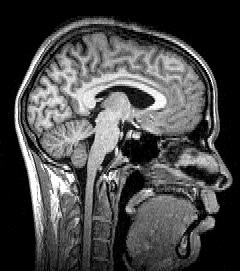
\includegraphics[height=0.618\textheight]{./images/Sagittal_brain_MRI}
				\source{w.wiki/7g4}{\ccbysa}
			}
			\only<3|handout:2>{%
				\begin{tikzpicture}[remember picture,overlay]%
					\node at (current page.center){%
						\mode<beamer>{\animategraphics[loop,autoplay,width=\paperwidth,every=\everyframe]{24}{./movies/mouse_skull/mouse_skull}{000}{236}}
						\mode<handout>{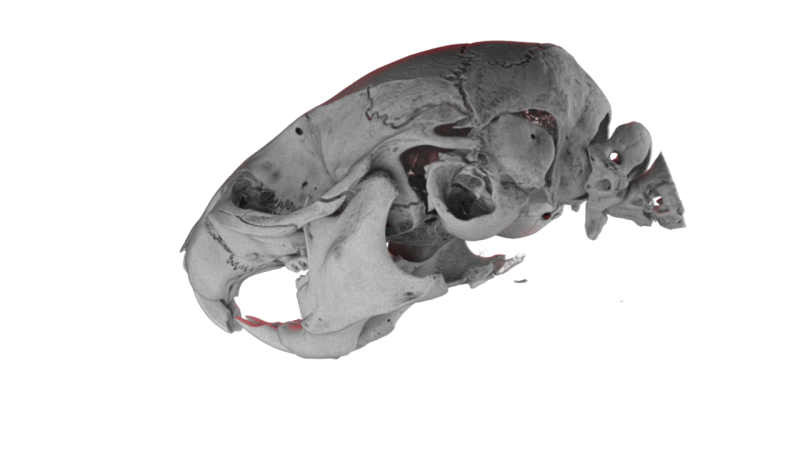
\includegraphics[width=\paperwidth]{./movies/mouse_skull/mouse_skull075}}
					};%
				\end{tikzpicture}%
			}
		\end{column}
	\end{columns}
\end{frame}

\section{Imaging}
\begin{frame}{Wavelength \& Scale}
	\centering
	\only<1|handout:1>{%
		\includegraphics[height=\imheight]{./images/2000px-Electromagnetic_spectrum_with_sources}%
		\source{w.wiki/7fz}{\ccbysa}%
		}%
	\only<2|handout:2>{%
		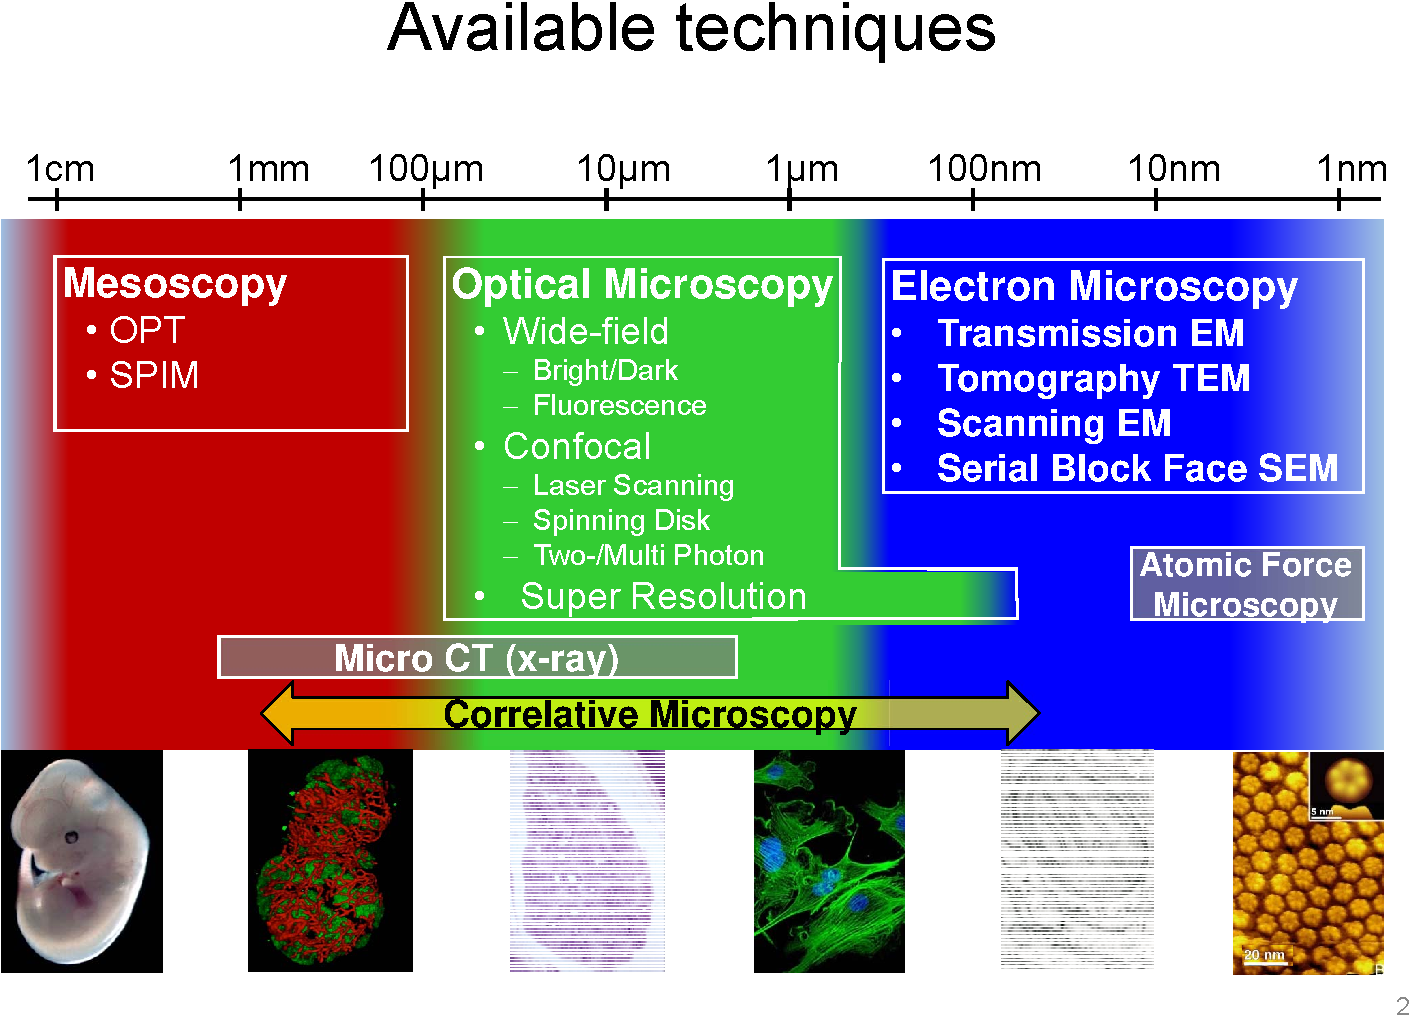
\includegraphics[height=\imheight]{./images/AnatomySeminarYuryBelyaev-cropped}%
		\sourcelink{www.mic.unibe.ch/organisation.php}{Yury Belyaev, MIC}{slide from internal seminar presentation}%
		}
\end{frame}

\begin{frame}{Imaging methods}
	\begin{itemize}
		\item Light microscopy: see \href{https://ilias.unibe.ch/goto_ilias3_unibe_sess_1555739.html}{lecture of Nadia Mercader Huber}
		\item X-ray imaging
		\item Electron microscopy: see lectures
			\href{https://ilias.unibe.ch/goto_ilias3_unibe_sess_1555738.html}{\emph{Transmission Electron Microscopy} by Dimitri Vanhecke},
			\href{https://ilias.unibe.ch/goto_ilias3_unibe_sess_1555742.html}{\emph{Scanning Electron Microscopy} by Michael Stoffel} and
			\href{https://ilias.unibe.ch/goto_ilias3_unibe_sess_1555743.html}{\emph{Cryoelectron Microscopy \& Serial Block Face SEM} by Ioan Iacovache}.
	\end{itemize}
\end{frame}

\section{Tomography}
\begin{frame}{CT-Scanner}
	\centering
	\mode<beamer>{%
		\animategraphics[loop,autoplay,height=0.618\textheight,every=\everyframe]{24}{./movies/ct-scanner/ct-scanner0}{001}{480}%
		\source{youtu.be/2CWpZKuy-NE}{}%
		}
	\mode<handout>{%
		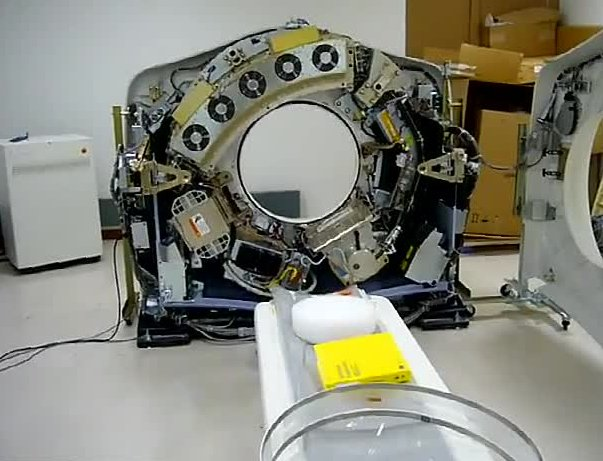
\includegraphics[height=0.618\textheight]{./movies/ct-scanner/ct-scanner0001}%
		\source{youtu.be/2CWpZKuy-NE}{}%
		}
	\note{From \href{https://www.bruker.com/products/microtomography/micro-ct-for-sample-scanning/x-ray-micro-ct-microtomography.html}:
		Micro computed tomography or micro-CT is x-ray imaging in 3D, by the same method used in hospital CT (or CAT) scans, but on a small scale with massively increased resolution.
		It really represents 3D microscopy, where very fine scale internal structure of objects is imaged non-destructively.
		No sample preparation, no staining, no thin slicing - a single scan will image your sample's complete internal 3D structure at high resolution, plus you get your intact sample back at the end!}
\end{frame}

\subsection{History}
\renewcommand{\imwidth}{\columnwidth}
\begin{frame}{History}
	\begin{columns}
		\begin{column}{0.49\linewidth}
			\begin{itemize}
				\item<1-|handout:1-> Long history 
				\begin{itemize}
					\item<1-|handout:1-> \citeyear{Cormack1963}: \citeauthor{Cormack1963} used a collimated \ce{^{60}Co} source and a Geiger counter as a detector~\cite{Cormack1963}
					\item<1-|handout:1-> \citeyear{Hounsfield1976a}: \citeauthor{Hounsfield1976a} worked on first clinical scanner~\cite{Hounsfield1976a}
					\item<1-|handout:1-> Nice overview by \citeauthor{Hsieh2003}~\cite{Hsieh2003}
				\end{itemize}
				\item<1-|handout:1-> First, second and third generation of scanners
			\end{itemize}
		\end{column}
		\begin{column}{0.49\linewidth}
			\centering
			\includegraphics<1|handout:1>[width=\imwidth]{./images/History_Generation1}%
			\only<1|handout:1>{\sourcecite{Hsieh2003}{Figure 1.12}}%
			\includegraphics<2|handout:2>[width=\imwidth]{./images/History_Generation2}%
			\only<2|handout:2>{\sourcecite{Hsieh2003}{Figure 1.13}}%
			\includegraphics<3|handout:3>[width=\imwidth]{./images/History_Generation3}%
			\only<3|handout:3>{\sourcecite{Hsieh2003}{Figure 1.14}}%
		\end{column}
	\end{columns}
\end{frame}

\subsection{Interaction of x-rays with matter}
\begin{frame}{X-ray interaction}
	\begin{itemize}
		\item \textquote[\cite{xrayphysics}]{X-rays interact with tissue in 2 main ways: photoelectric effect and Compton scatter.
				To a first approximation, the photoelectric effect contributes to contrast while the Compton effect contributes to noise.
				Both contribute to dose.}
		\begin{itemize}
			\item Photoelectric absorption (\(\tau\)) is strongly dependent on the atomic number \(Z\) of the absorbing material: \(\tau\propto\frac{Z^4}{E^{3.5}}\)
			\note{From \href{https://radiopaedia.org/articles/photoelectric-effect}{Radiopaedia.org}: Therefore if \(Z\) doubles, PEA will increase by a factor of 16 (\(2^4=8\)), and if \(E\) doubles PEA will reduce by a factor of 16.
				Small changes in \(Z\) and \(E\) can therefore significantly affect PEA.
				This has practical implications in the field of radiation protection and is the reason why materials with a high \(Z\) such as lead (\(Z= 82\)) are useful shielding materials.
				The dependence of PEA on \(Z\) and \(E\) means that it is the major contributor to beam attenuation up to approximately 30 keV when human tissues (\(Z=7.4\)) are irradiated.
				At beam energies above this, the Compton effect predominates.}
			\item Compton scattering is one of the principle forms of photon interaction and is directly proportional to the (electron \& physical) density of the material.
				It does \emph{not} depend on the atomic number: \(\lambda' - \lambda = \frac{h}{m_e c}\left(1-\cos{\theta}\right)\)
			\note{Where \(\lambda\) is the initial wavelength, \(\lambda'\) is the wavelength after scattering, \(h\) is the Planck constant, \(m_e\) is the electron rest mass, \(c\) is the speed of light, and \(\theta\) is the scattering angle.}
		\end{itemize}
		\item Lowering x-ray energy increases contrast
		\item X-ray penetration decreases exponentially with sample thickness (\cite[\ie Beer-Lamberts law]{wiki:beer-lambert} \(I(t) = I_0 \, e^{-\alpha z}\)
	\end{itemize}
\end{frame}

\begin{frame}{Composition of biological tissues}
	Tissue: content by mass percentage
	\centering
	\begin{table}
		\only<1>{%
			\pgfplotstabletypeset[%
				col sep=comma, % the seperator in our .csv file
				display columns/0/.style={string type,column name={Element}},
				% section 3.2 in pgfplotstable manual
				every head row/.style={before row={\toprule}},
				every row no 0/.style={after row=\midrule},
				every last row/.style={after row=\bottomrule},
			]{./tables/tissue-composition.csv}
		}
		\only<2|handout:0>{%
			\pgfplotstabletypeset[%
				col sep=comma, % the seperator in our .csv file
				display columns/0/.style={string type,column name={Element}},
				every head row/.style={before row={\toprule}},
				every row no 0/.style={after row=\midrule},
				every last row/.style={after row=\bottomrule},
				% make certain cells ubRed, based on https://tex.stackexchange.com/a/296914/828
				every row 1 column 2/.style={postproc cell content/.append style={/pgfplots/table/@cell content/.add={\cellcolor{ubRed!61.8}}{}}},
				every row 1 column 4/.style={postproc cell content/.append style={/pgfplots/table/@cell content/.add={\cellcolor{ubRed!61.8}}{}}},
				every row 6 column 6/.style={postproc cell content/.append style={/pgfplots/table/@cell content/.add={\cellcolor{ubRed!61.8}}{}}},
				every row 6 column 10/.style={postproc cell content/.append style={/pgfplots/table/@cell content/.add={\cellcolor{ubRed!61.8}}{}}}
			]{./tables/tissue-composition.csv}
		}
	\end{table}
	\note{Bone, lean tissue, fat and air can be distinguished quite easily}	
\end{frame}


\renewcommand{\imwidth}{\columnwidth}
\begin{frame}[label=current]{Why \uct?}
	\begin{columns}
		\begin{column}{0.49\linewidth}
			% https://www.cancerimagingarchive.net/nbia-search/?saved-cart=nbia-76761575299081509
			\only<1-4|handout:1-4>{%
				\pgfmathsetlength{\imagewidth}{\imwidth}%
				\pgfmathsetlength{\imagescale}{\imagewidth/512}%
				\def\x{316}% scalebar-x starting at golden ratio of image width of 512px = 316
				\def\y{361}% scalebar-y at 90% of image height of 401px = 361
				\begin{tikzpicture}[x=\imagescale,y=-\imagescale]
					\node[anchor=north west, inner sep=0pt, outer sep=0pt] at (0,0) {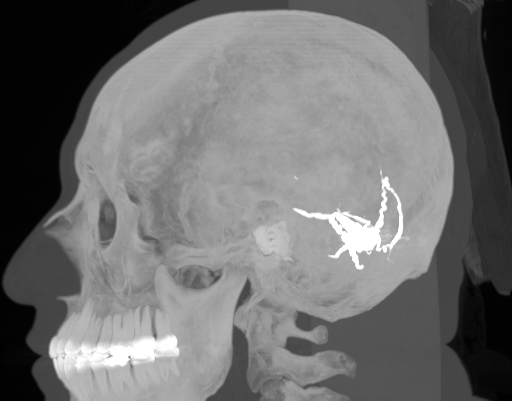
\includegraphics[width=\imagewidth]{./images/comparison/MAX_human}};
					% 512.000px = 250.0096mm -> 100px = 48830.000um -> 1.024px = 500um, 0.205px = 100um
					%\draw[|-|,blue,thick] (0,200) -- (512,200) node [sloped,midway,above,fill=white,semitransparent,text opacity=1] {\SI{250.0096}{\milli\meter} (512px) TEMPORARY!};
					\draw[|-|,white,shadowed] (\x,\y) -- (\x+102.4,\y) node [midway,above] {\shadowtext{\SI{5}{\centi\meter}}};
				\end{tikzpicture}%
			}%
			\only<5|handout:0>{%
				\pgfmathsetlength{\imagewidth}{\imwidth}%
				\pgfmathsetlength{\imagescale}{\imagewidth/512}%
				\def\x{316}% scalebar-x starting at golden ratio of image width of 512px = 316
				\def\y{361}% scalebar-y at 90% of image height of 401px = 361
				\def\mag{5}% magnification of inset
				\def\size{100}% size of inset
				\begin{tikzpicture}[x=\imagescale,y=-\imagescale,spy using outlines={rectangle,magnification=\mag,size=\size,connect spies}]
					\node[anchor=north west, inner sep=0pt, outer sep=0pt] at (0,0) {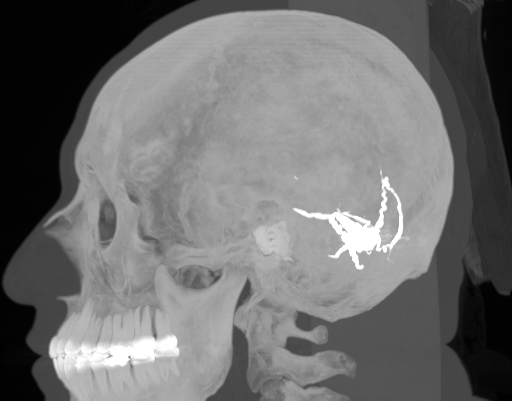
\includegraphics[width=\imagewidth]{./images/comparison/MAX_human}};
					\spy [red] on (102,342) in node at (256,201) [anchor=center];
					% 512.000px = 250.0096mm -> 100px = 48830.000um -> 1.024px = 500um, 0.205px = 100um
					\draw[|-|,white,shadowed] (\x,\y) -- (\x+102.4,\y) node [midway,above] {\shadowtext{\SI{5}{\centi\meter}}};
				\end{tikzpicture}%
			}%
			\renewcommand{\imwidth}{0.1554\columnwidth}%			
			\only<6|handout:5>{%
				\centering
				\pgfmathsetlength{\imagewidth}{\imwidth}%
				\pgfmathsetlength{\imagescale}{\imagewidth/512}%
				\def\x{316}% scalebar-x starting at golden ratio of image width of 512px = 316
				\def\y{361}% scalebar-y at 90% of image height of 401px = 361
				\begin{tikzpicture}[x=\imagescale,y=-\imagescale]
					\node[anchor=north west, inner sep=0pt, outer sep=0pt] at (0,0) {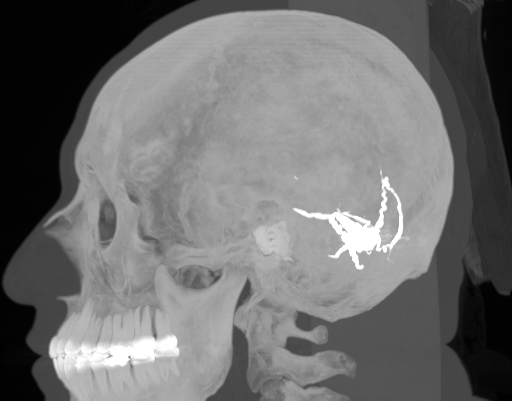
\includegraphics[width=\imagewidth]{./images/comparison/MAX_human}};
					% 512.000px = 250.0096mm -> 100px = 48830.000um -> 1.024px = 500um, 0.205px = 100um
					\draw[|-|,white,shadowed] (\x,\y) -- (\x+102.4,\y) node [midway,above] {\shadowtext{\SI{5}{\centi\meter}}};
				\end{tikzpicture}%
			}%			
			\sourcecite{Clark2013}{Subject \emph{C3L-02465}}
		\end{column}%
		\begin{column}{0.49\linewidth}
			\only<1|handout:1>{%
				\pgfmathsetlength{\imagewidth}{\imwidth}%
				\pgfmathsetlength{\imagescale}{\imagewidth/3295}%
				\def\x{2036}% scalebar-x starting at golden ratio of image width of 3295px = 2036
				\def\y{1343}% scalebar-y at 90% of image height of 1492px = 1343
				\begin{tikzpicture}[x=\imagescale,y=-\imagescale]
					\node[anchor=north west, inner sep=0pt, outer sep=0pt] at (0,0) {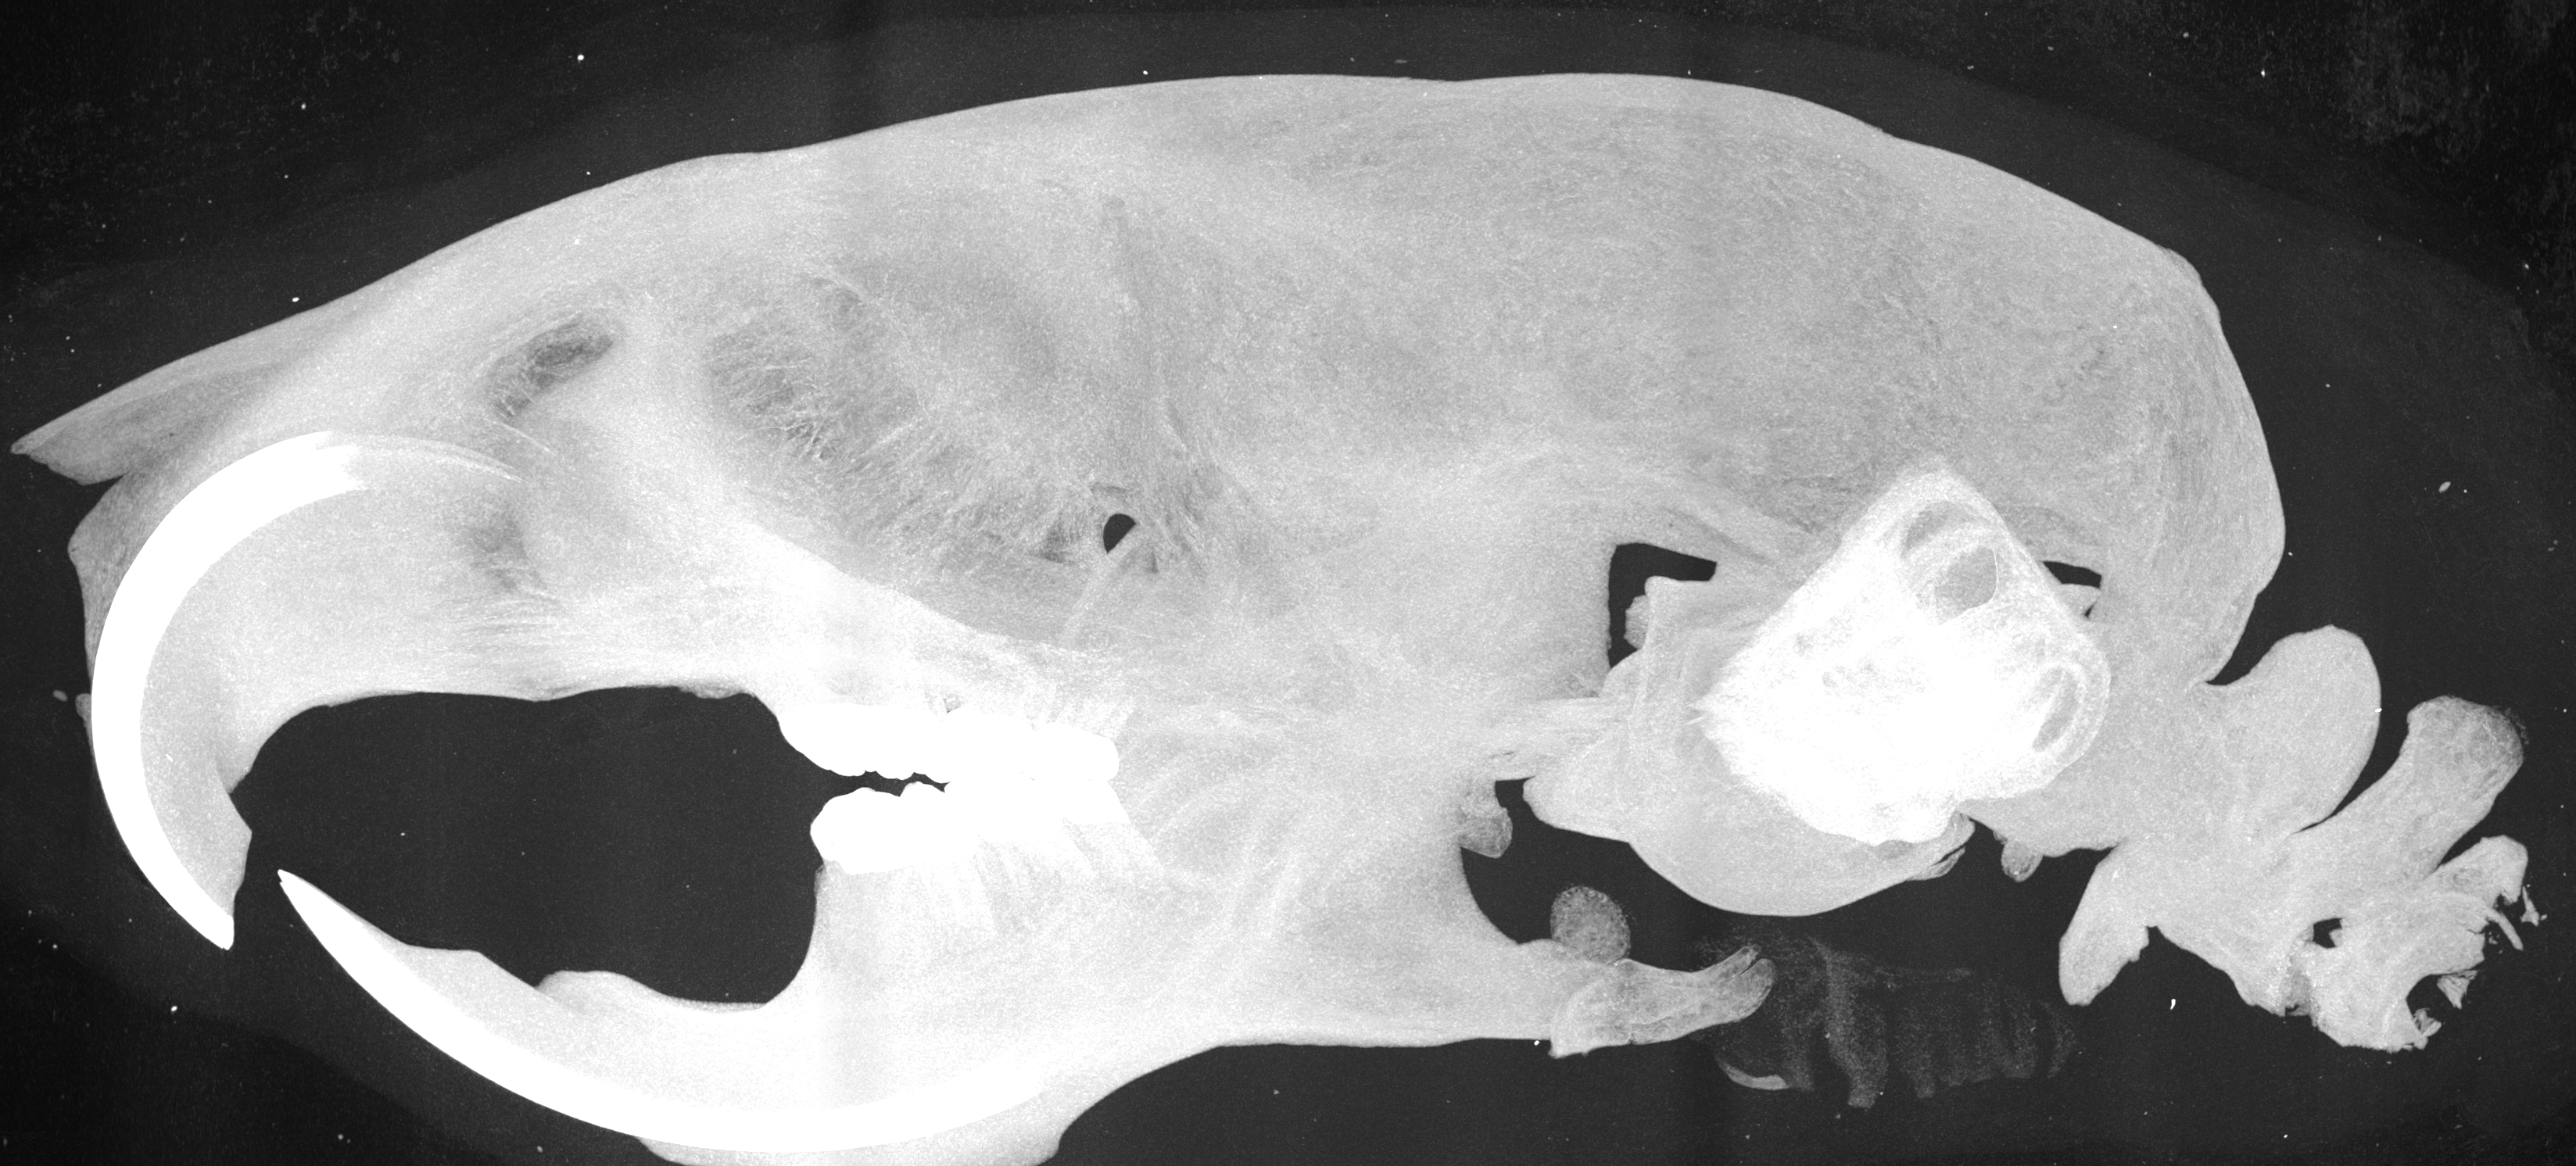
\includegraphics[width=\imagewidth]{./images/comparison/MAX_mouse}};
					% 3295.000px = 26.2282mm -> 100px = 796.000um -> 62.814px = 500um, 12.563px = 100um
					%\draw[|-|,blue,thick] (0,746) -- (3295,746) node [sloped,midway,above,fill=white,semitransparent,text opacity=1] {\SI{26.2282}{\milli\meter} (3295px) TEMPORARY!};
					\draw[|-|,white,shadowed] (\x,\y) -- (\x+628.14,\y) node [midway,above] {\shadowtext{\SI{5}{\milli\meter}}};
				\end{tikzpicture}%
			}%
			\renewcommand{\imwidth}{0.1\columnwidth}%
			\only<2|handout:2>{%
				\centering
				\pgfmathsetlength{\imagewidth}{\imwidth}%
				\pgfmathsetlength{\imagescale}{\imagewidth/54}%
				\def\x{33}% scalebar-x starting at golden ratio of image width of 54px = 33
				\def\y{22}% scalebar-y at 90% of image height of 24px = 22
				\begin{tikzpicture}[x=\imagescale,y=-\imagescale]
					\node[anchor=north west, inner sep=0pt, outer sep=0pt] at (0,0) {
\includegraphics[width=\imagewidth]{./images/comparison/MAX_mouse_488umppx}};
					% 54.000px = 26.3682mm -> 100px = 48830.000um -> 1.024px = 500um, 0.205px = 100um
					%\draw[|-|,blue,thick] (0,12) -- (54,12) node [sloped,midway,above,fill=white,semitransparent,text opacity=1] {\SI{26.3682}{\milli\meter} (54px) TEMPORARY!};
					\draw[|-|,white,shadowed] (\x,\y) -- (\x+102.4,\y) node [midway,above] {\shadowtext{\SI{5}{\centi\meter}}};
					%\draw[color=red, anchor=south west] (0,24) node [fill=white, semitransparent] {Legend} node {Legend};
				\end{tikzpicture}%
			}%
			\renewcommand{\imwidth}{\columnwidth}
			\only<3|handout:3>{%
				\centering
				\pgfmathsetlength{\imagewidth}{\imwidth}%
				\pgfmathsetlength{\imagescale}{\imagewidth/54}%
				\def\x{33}% scalebar-x starting at golden ratio of image width of 54px = 33
				\def\y{22}% scalebar-y at 90% of image height of 24px = 22
				\begin{tikzpicture}[x=\imagescale,y=-\imagescale]
					\node[anchor=north west, inner sep=0pt, outer sep=0pt] at (0,0) {
\includegraphics[width=\imagewidth]{./images/comparison/MAX_mouse_488umppx}};
					% 54.000px = 26.3682mm -> 100px = 48830.000um -> 1.024px = 500um, 0.205px = 100um
					%\draw[|-|,blue,thick] (0,12) -- (54,12) node [sloped,midway,above,fill=white,semitransparent,text opacity=1] {\SI{26.3682}{\milli\meter} (54px) TEMPORARY!};
					\draw[|-|,white,shadowed] (\x,\y) -- (\x+10.24,\y) node [midway,above] {\shadowtext{\SI{5}{\milli\meter}}};
					%\draw[color=red, anchor=south west] (0,24) node [fill=white, semitransparent] {Legend} node {Legend};
				\end{tikzpicture}%
			}%
			\only<4|handout:4>{%
				\pgfmathsetlength{\imagewidth}{\imwidth}%
				\pgfmathsetlength{\imagescale}{\imagewidth/3295}%
				\def\x{2036}% scalebar-x starting at golden ratio of image width of 3295px = 2036
				\def\y{1343}% scalebar-y at 90% of image height of 1492px = 1343
				\begin{tikzpicture}[x=\imagescale,y=-\imagescale]
					\node[anchor=north west, inner sep=0pt, outer sep=0pt] at (0,0) {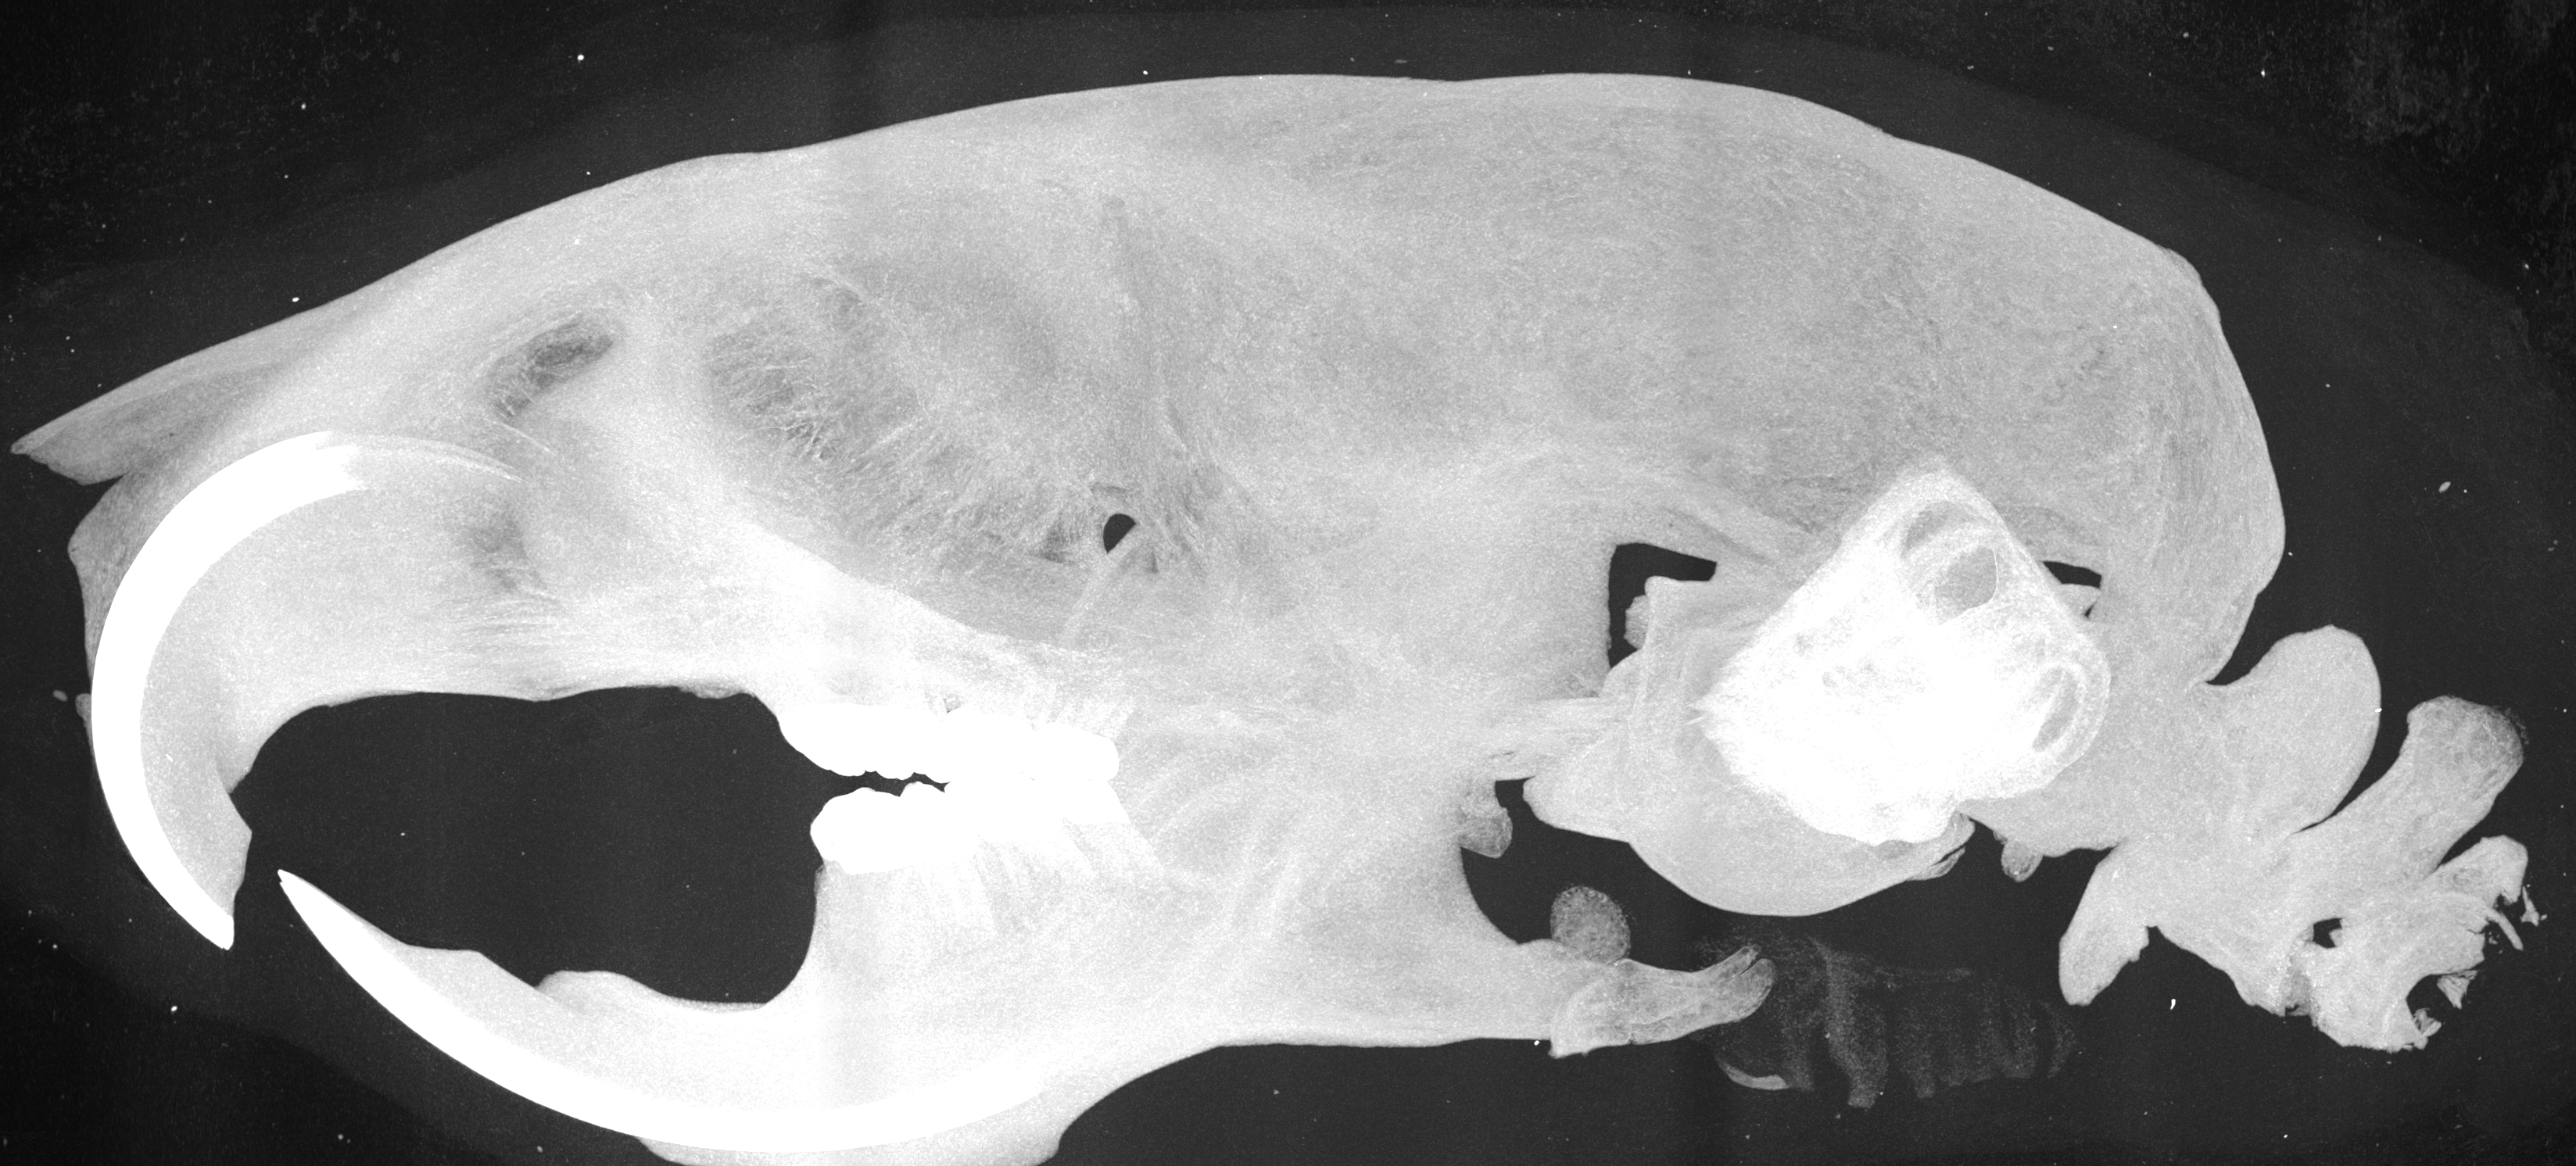
\includegraphics[width=\imagewidth]{./images/comparison/MAX_mouse}};
					% 3295.000px = 26.2282mm -> 100px = 796.000um -> 62.814px = 500um, 12.563px = 100um
					\draw[|-|,white,shadowed] (\x,\y) -- (\x+628.14,\y) node [midway,above] {\shadowtext{\SI{5}{\milli\meter}}};
				\end{tikzpicture}%
			}%
			\only<5|handout:0>{%
				\pgfmathsetlength{\imagewidth}{\imwidth}%
				\pgfmathsetlength{\imagescale}{\imagewidth/3295}%
				\def\x{2036}% scalebar-x starting at golden ratio of image width of 3295px = 2036
				\def\y{1343}% scalebar-y at 90% of image height of 1492px = 1343
				\def\mag{5}% magnification of inset
				\def\size{100}% size of inset
				\begin{tikzpicture}[x=\imagescale,y=-\imagescale,spy using outlines={rectangle,magnification=\mag,size=\size,connect spies}]
					\node[anchor=north west, inner sep=0pt, outer sep=0pt] at (0,0) {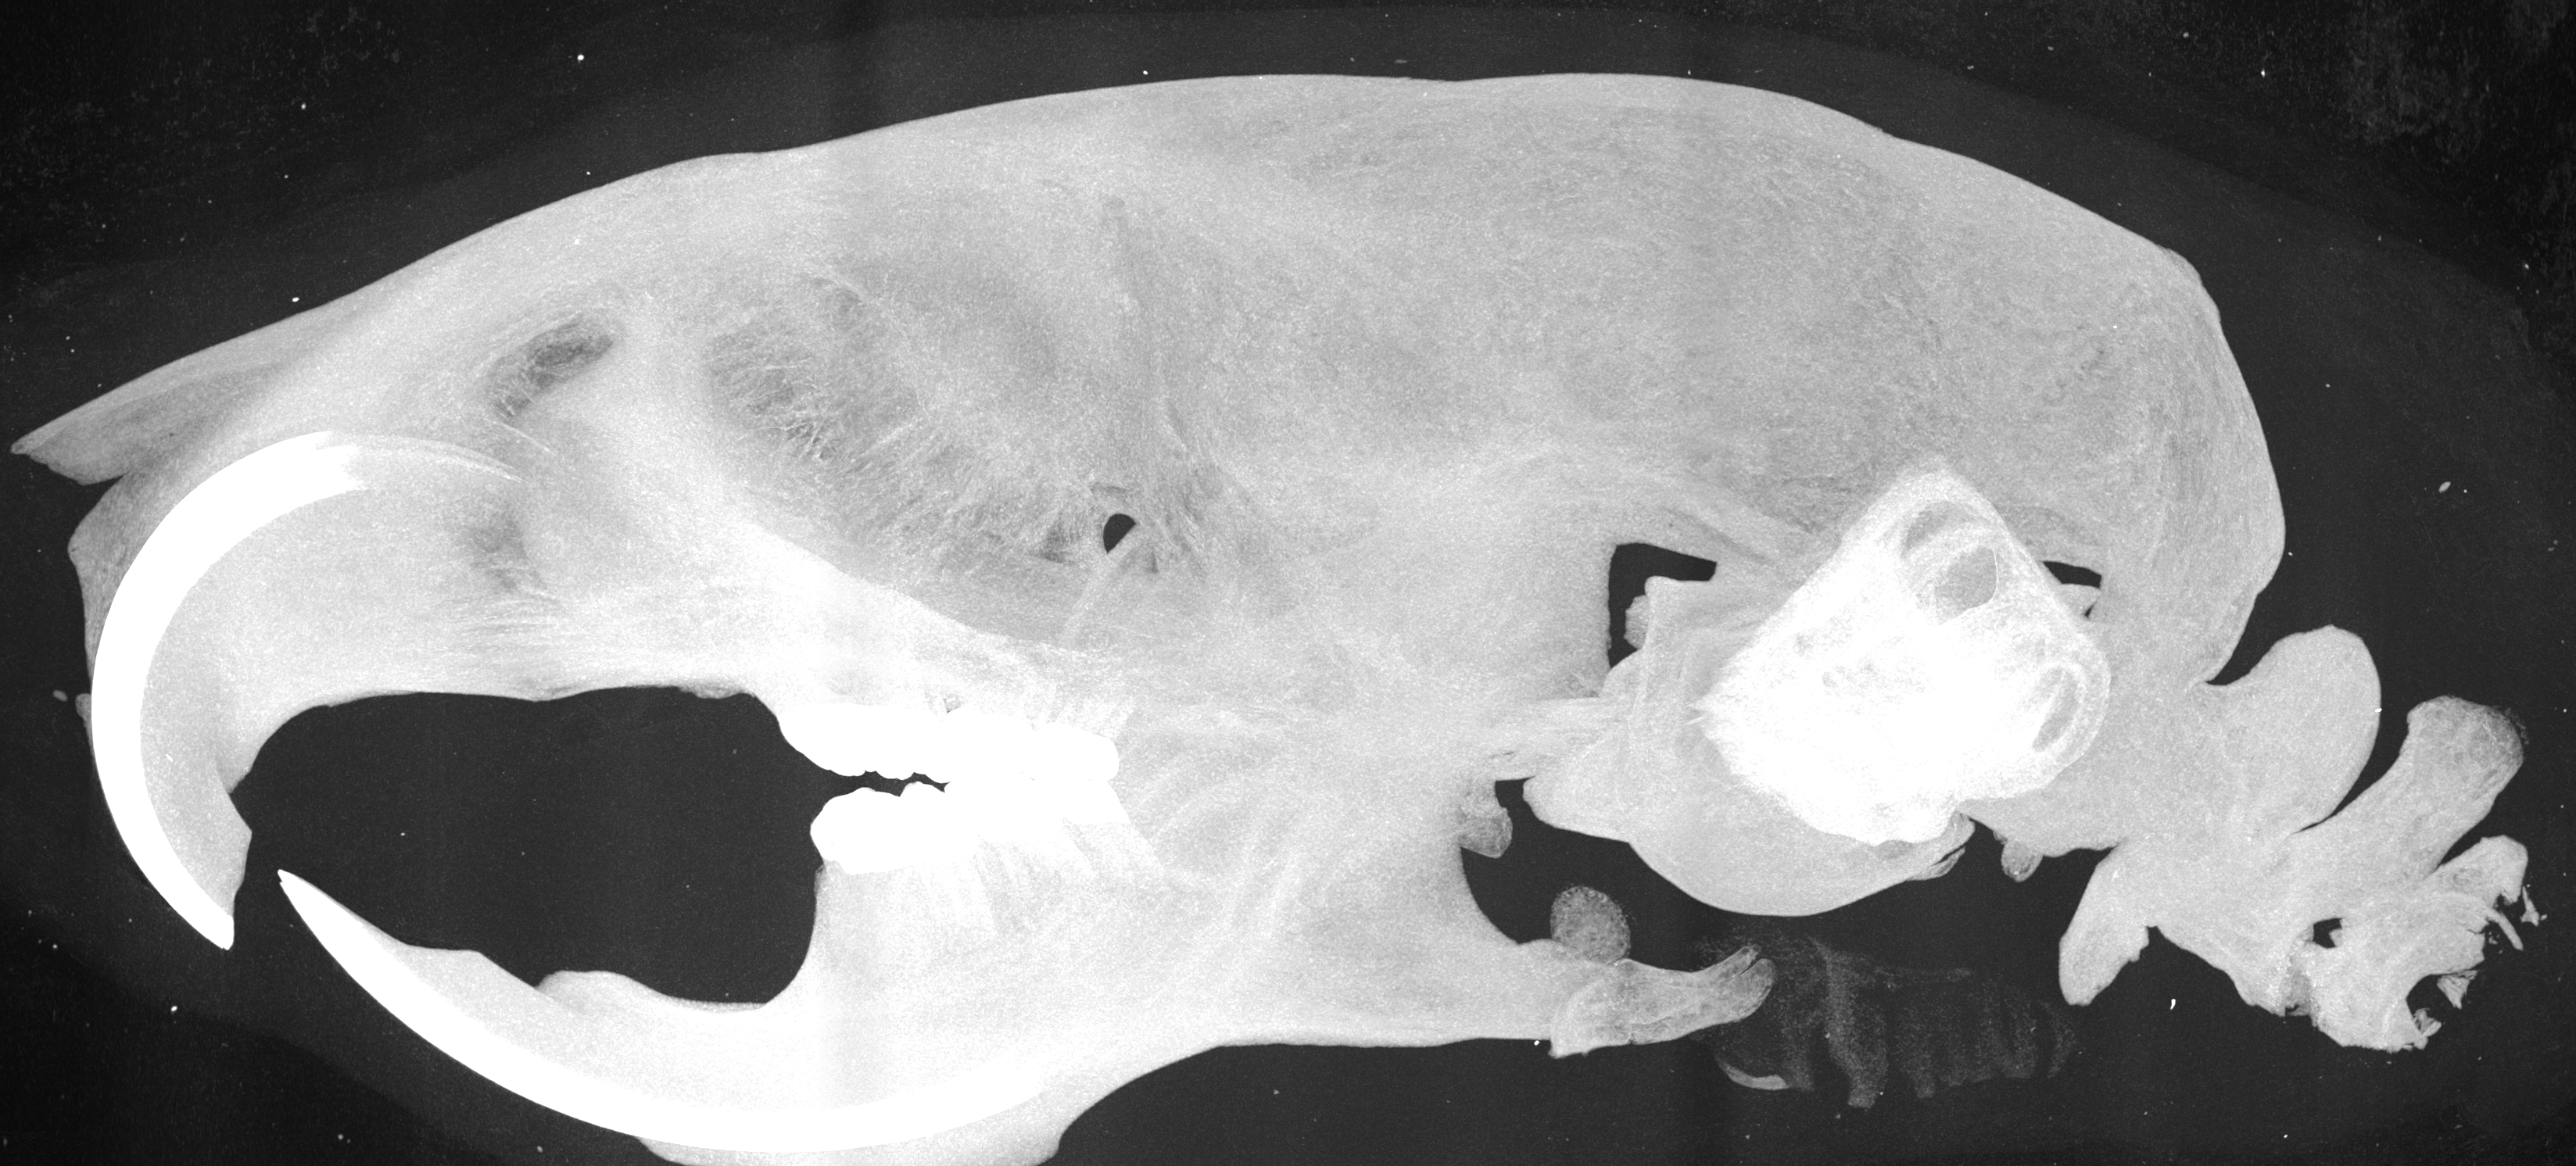
\includegraphics[width=\imagewidth]{./images/comparison/MAX_mouse}};
					\spy [red] on (352,1116) in node at (1648,746) [anchor=center];
					% 3295.000px = 26.2282mm -> 100px = 796.000um -> 62.814px = 500um, 12.563px = 100um
					\draw[|-|,white,shadowed] (\x,\y) -- (\x+628.14,\y) node [midway,above] {\shadowtext{\SI{5}{\milli\meter}}};
				\end{tikzpicture}%
			}%
			\only<6|handout:5>{%
				\pgfmathsetlength{\imagewidth}{\imwidth}%
				\pgfmathsetlength{\imagescale}{\imagewidth/3295}%
				\def\x{2036}% scalebar-x starting at golden ratio of image width of 3295px = 2036
				\def\y{1343}% scalebar-y at 90% of image height of 1492px = 1343
				\begin{tikzpicture}[x=\imagescale,y=-\imagescale]
					\node[anchor=north west, inner sep=0pt, outer sep=0pt] at (0,0) {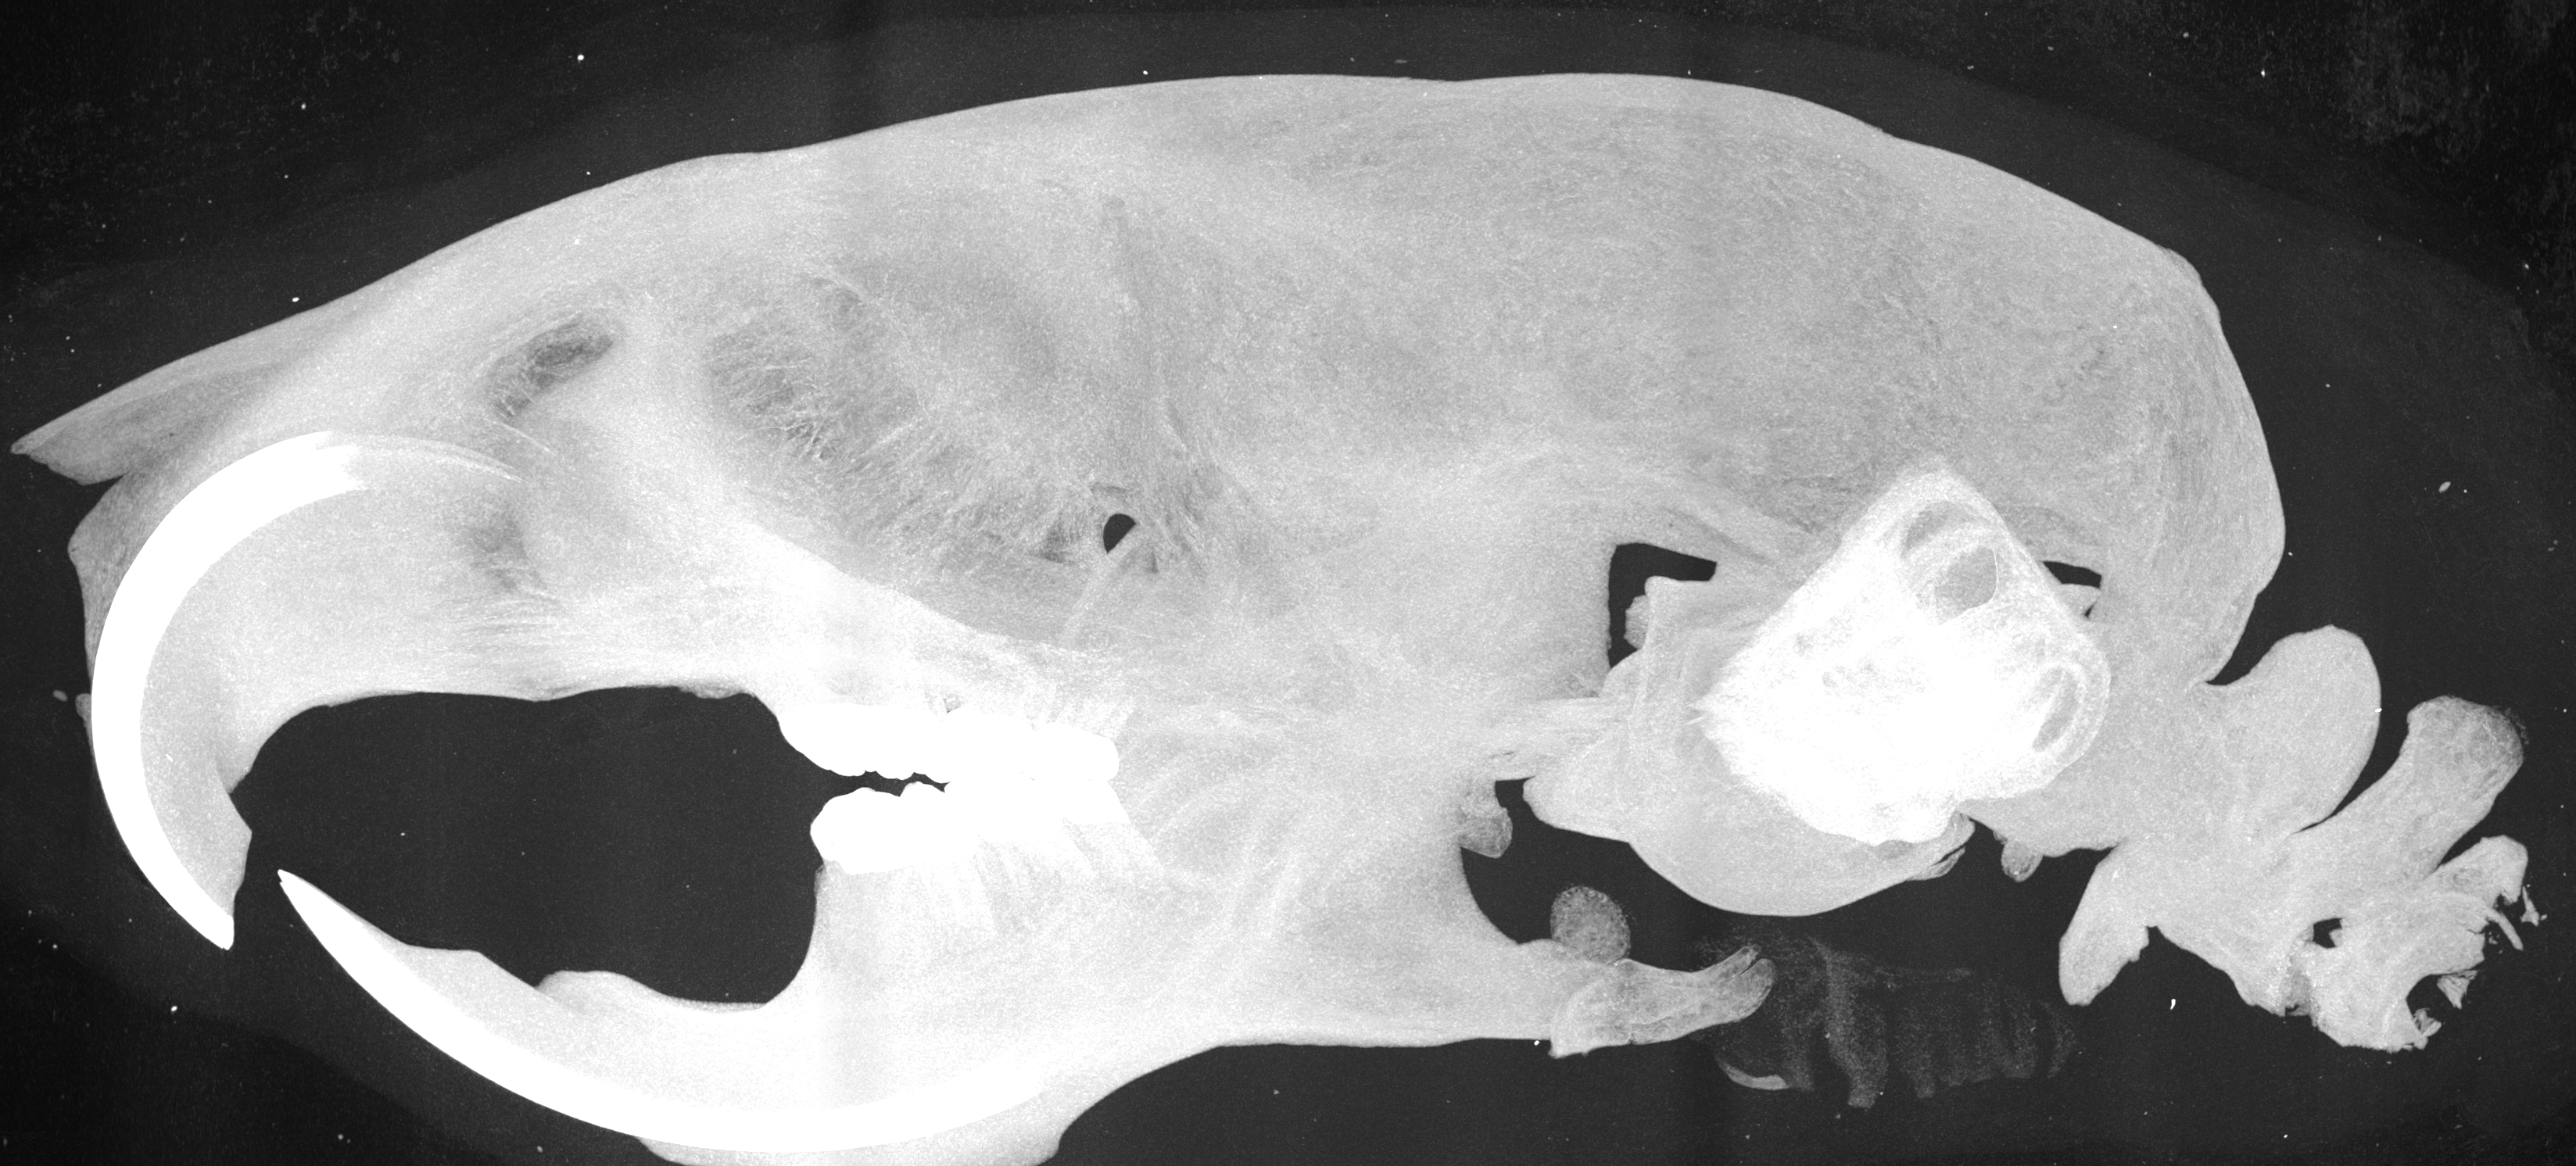
\includegraphics[width=\imagewidth]{./images/comparison/MAX_mouse}};
					% 3295.000px = 26.2282mm -> 100px = 796.000um -> 62.814px = 500um, 12.563px = 100um
					\draw[|-|,white,shadowed] (\x,\y) -- (\x+628.14,\y) node [midway,above] {\shadowtext{\SI{5}{\milli\meter}}};
				\end{tikzpicture}%
			}%
		\end{column}
	\end{columns}
\end{frame}
\note{The human head scan was downloaded from the \href{https://www.cancerimagingarchive.net}{[Cancer Imaging Archive}{Cancer Imaging Archive}.
	We loaded the DICOM slices in Fiji, resliced it to show it from the side and then used to generate an MIP.
	According to the DICOM tags, the voxel size is \SI{0.4883x0.4883x0.625}{\milli\meter\cubed}, the image size is 512\(\times\)512 pixels.
	The mouse head is the same as shown in the early animation.
	The files from the early animation are resized 0.25 times, so we used the original dataset (Mouse1265\_Skull\_Gaby\_TKI\_7\_96um\_Al05\_2K) for a reslice and the generation of the MIP.
	The voxel size of the original data is 7.96 um, the image size is 3295\(\times\)1492 pixels.
	}

\subsection{Tomography today}
\begin{frame}{Machinery}
	\begin{columns}
		\begin{column}{0.4\linewidth}
			\begin{itemize}
				\item<1-> Hospital CT
				\begin{itemize}
					\item Voxel size around \SI{0.5}{\milli\meter}
				\end{itemize}
				\item<2-> Lab/Desktop CT
				\begin{itemize}
					\item Voxel size around \SI{7}{\micro\meter} (\emph{in vivo}) or \SI{0.5}{\micro\meter} (\emph{ex vivo})
				\end{itemize}
				\item<4-> Synchrotron CT
				\begin{itemize}
					\item Voxel size down to \href{https://www.psi.ch/en/sls/tomcat/detectors}{\SI{160}{\nano\meter}}
				\end{itemize}
			\end{itemize}
		\end{column}
		\begin{column}{0.6\linewidth}
			\centering
			\includegraphics<1|handout:1>[height=\imheight]{./images/24324062640_751e011e1a_o}%
			\only<1|handout:1>{\source{flic.kr/p/D4rbom}{\ccbyncsa}}
			\includegraphics<2|handout:2>[width=\imheight]{./images/9459311320_516179207a_o}%
			\only<2|handout:2>{\source{flic.kr/p/fpTrGu}{\ccbysa}}
			\includegraphics<3|handout:3>[width=\imwidth]{./images/1272}%
			\only<3|handout:3>{\source{bruker.com/skyscan1272}{}}
			\includegraphics<4|handout:4>[width=\imwidth]{./images/4563733710_f632792416_b}%
			\only<4|handout:4>{\source{flic.kr/p/7Xhk2Y}{\ccbync}}
		\end{column}
	\end{columns}
\end{frame}
\note{FAN BEAM -> BRUKER\newline
	PARALLEL BEAM -> TOMCAT\newline
	HELICAL/SPIRAL CT\newline
	MULTISLICE CT -> HOSPITAL
}

\begin{frame}{Machinery}
	No matter what kind of machine, the basic principle is always the same
	\begin{itemize}
		\item an x-ray source
		\item a sample
		\item a detector
	\end{itemize}
\end{frame}

\begin{frame}{Machinery}
	\begin{columns}
		\begin{column}{0.49\linewidth}
			\centering
			\documentclass{standalone}
% Draw the setup where the source and detector move, e.g. classic CT
% With help from https://tex.stackexchange.com/q/515519/828
\usepackage{animate}
\usepackage{tikz}
%	\usetikzlibrary{external}
%	\tikzexternalize
%	\tikzsetnextfilename{classicCT}
\usepackage{fontawesome5}	
\usepackage{ifthen}
\ifthenelse{\isundefined{\everyframe}}{%
	% If we're compiling this file via \input, then these variables are already defined.
	% In the other case, we need to define them
	\newcommand{\everyframe}{5}
	\definecolor{ubRed}{HTML}{E6002E}
	% split complementary images from https://www.sessions.edu/color-calculator/
	\definecolor{ubRedComplementary1}{HTML}{00a1e6}
	\definecolor{ubRedComplementary2}{HTML}{00e645}
	\definecolor{ubGrey}{RGB}{217,217,217}
	}{}
\begin{document}
\begin{animateinline}[every=\everyframe,loop]{25}
	\multiframe{180}{n=1+2}{%
%	\tikzifexternalizing{Work-around to make animate happy	}{}%https://tex.stackexchange.com/a/39026/828
		\begin{tikzpicture}
			\pgfdeclarelayer{background}
			\pgfsetlayers{background,main}
			%Help lines
			\draw[<->] (-2.25,0) -- (2.25,0);
			\draw[<->] (0,-2.25) -- (0,2.25);
			\draw[help lines,step=1cm,ultra thin] (-2.45,-2.45) grid (2.45,2.45);
			% Stuff that stays put
			\node[ubRedComplementary1] at (0,0) (sample) {\Huge\faUser};
			% Stuff that moves
			\mode<beamer>{%
				\begin{scope}[rotate around={\n:(sample)}]
				}
				% Rotation arc
				\draw[->, thick,line cap=rect] (1.5,0) arc [start angle=0, end angle=180, radius=1.5];
				\draw[->, thick,line cap=rect] (-1.5,0) arc [start angle=-180, end angle=0, radius=1.5];
				% Source
				\fill[ubRed] (-0.25,1.5) rectangle node (source) [black] {X-ray} +(0.5,0.5);
				% Detector and detector edges
				\fill[ubRedComplementary2,fill] (-0.5,-1.75) rectangle node (detector) [black] {Detector} +(1,0.25);
				\coordinate (dl) at (-0.45,-1.75);
				\coordinate (dr) at (0.45,-1.75);
				% X-ray cone
				\begin{pgfonlayer}{background}
					\fill[gray,semitransparent] (source.center) -- (dl) -- (dr) -- cycle;
				\end{pgfonlayer}
			\mode<beamer>{%
				\end{scope}
			}
		\end{tikzpicture}
	}
\end{animateinline}
\end{document}

		\end{column}
		\begin{column}{0.49\linewidth}
			\centering
			\only<1>{\documentclass{standalone}
% Draw the setup where the only the sample moves, e.g. microCT
% Essentially just a copy of classicCT in the same folder
\usepackage{animate}
\usepackage{tikz}
%	\usetikzlibrary{external}
%	\tikzexternalize
%	\tikzsetnextfilename{microCT}
\usepackage{fontawesome5}	
\usepackage{ifthen}
\ifthenelse{\isundefined{\everyframe}}{%
	% If we're compiling this file via \input, then these variables are already defined.
	% In the other case, we need to define them
	\newcommand{\everyframe}{5}
	\definecolor{ubRed}{HTML}{E6002E}
	% split complementary images from https://www.sessions.edu/color-calculator/
	\definecolor{ubRedComplementary1}{HTML}{00a1e6}
	\definecolor{ubRedComplementary2}{HTML}{00e645}
	\definecolor{ubGrey}{RGB}{217,217,217}
	}{}
\begin{document}
\begin{animateinline}[every=\everyframe,loop]{25}
	\multiframe{180}{n=1+2}{%
%	\tikzifexternalizing{Work-around to make animate happy	}{}%https://tex.stackexchange.com/a/39026/828
		\begin{tikzpicture}
			\pgfdeclarelayer{background}
			\pgfsetlayers{background,main}
			%Help lines
			\draw[<->] (-2.25,0) -- (2.25,0);
			\draw[<->] (0,-2.25) -- (0,2.25);
			\draw[help lines,step=1cm,ultra thin] (-2.45,-2.45) grid (2.45,2.45);
			% Stuff that stays put
			% Source
			\fill[ubRed] (-0.25,1) rectangle node (source) [black,opacity=0, text opacity=1] {X-ray} +(0.5,0.5);
			% Detector and detector edges
			\fill[ubRedComplementary2,fill] (-0.5,-1.25) rectangle node (detector) [black] {Detector} +(1,0.25);
			\coordinate (dl) at (-0.45,-1);
			\coordinate (dr) at (0.45,-1);
			% X-ray cone
			\begin{pgfonlayer}{background}
				\fill[gray,semitransparent] (source.center) -- (dl) -- (dr) -- cycle;
			\end{pgfonlayer}
			% Stuff that moves
			\mode<beamer>{%
				\begin{scope}[rotate around={\n:(0,0)}]
				}
				% Rotation arc
				\draw[->, thick,line cap=rect] (0.618,0) arc [start angle=0, end angle=180, radius=0.618];
				\draw[->, thick,line cap=rect] (-0.618,0) arc [start angle=-180, end angle=0, radius=0.618];
				% Sample
				\node[ubRedComplementary1] at (0,0) (sample) {\rotatebox{\n}{\Huge\faFish}};
			\mode<beamer>{%
				\end{scope}
				}
		\end{tikzpicture}
	}
\end{animateinline}
\end{document}
}%
			\only<2|handout:0>{\documentclass{standalone}
% Draw the setup where the only the sample moves, e.g. microCT
% Essentially just a copy of classicCT in the same folder
\usepackage{animate}
\usepackage{tikz}
%	\usetikzlibrary{external}
%	\tikzexternalize
%	\tikzsetnextfilename{microCT}
\usepackage{fontawesome5}	
\usepackage{ifthen}
\ifthenelse{\isundefined{\everyframe}}{%
	% If we're compiling this file via \input, then these variables are already defined.
	% In the other case, we need to define them
	\newcommand{\everyframe}{5}
	\definecolor{ubRed}{HTML}{E6002E}
	% split complementary images from https://www.sessions.edu/color-calculator/
	\definecolor{ubRedComplementary1}{HTML}{00a1e6}
	\definecolor{ubRedComplementary2}{HTML}{00e645}
	\definecolor{ubGrey}{RGB}{217,217,217}
	}{}
\begin{document}
\begin{animateinline}[every=\everyframe,loop]{25}
	\multiframe{180}{n=1+2}{%
%	\tikzifexternalizing{Work-around to make animate happy	}{}%https://tex.stackexchange.com/a/39026/828
		\begin{tikzpicture}
			\pgfdeclarelayer{background}
			\pgfsetlayers{background,main}
			%Help lines
			\draw[<->] (-2.25,0) -- (2.25,0);
			\draw[<->] (0,-2.25) -- (0,2.25);
			\draw[help lines,step=1cm,ultra thin] (-2.45,-2.45) grid (2.45,2.45);
			% Stuff that stays put
			% Source
			\fill[ubRed] (-0.25,1) rectangle node (source) [black,opacity=0, text opacity=1] {X-ray} +(0.5,0.5);
			% Detector and detector edges
			\fill[ubRedComplementary2,fill] (-0.5,-1.25) rectangle node (detector) [black] {Detector} +(1,0.25);
			\coordinate (dl) at (-0.45,-1);
			\coordinate (dr) at (0.45,-1);
			% X-ray cone
			\begin{pgfonlayer}{background}
				\fill[gray,semitransparent] (source.center) -- (dl) -- (dr) -- cycle;
			\end{pgfonlayer}
			% Stuff that moves
			\mode<beamer>{%
				\begin{scope}[rotate around={\n:(0,-0.5)}]
				}
				% Rotation arc
				\draw[->, thick,line cap=rect] (0.618,-0.5) arc [start angle=0, end angle=180, radius=0.618];
				\draw[->, thick,line cap=rect] (-0.618,-0.5) arc [start angle=-180, end angle=0, radius=0.618];
				% Sample
				\node[ubRedComplementary1] at (0,-0.5) (sample) {\rotatebox{\n}{\Huge\faFish}};
			\mode<beamer>{%
				\end{scope}
				}
		\end{tikzpicture}
	}
\end{animateinline}
\end{document}
}%
			\only<3|handout:0>{\documentclass{standalone}
% Draw the setup where the only the sample moves, e.g. microCT
% Essentially just a copy of classicCT in the same folder
\usepackage{animate}
\usepackage{tikz}
%	\usetikzlibrary{external}
%	\tikzexternalize
%	\tikzsetnextfilename{microCT}
\usepackage{fontawesome5}	
\usepackage{ifthen}
\ifthenelse{\isundefined{\everyframe}}{%
	% If we're compiling this file via \input, then these variables are already defined.
	% In the other case, we need to define them
	\newcommand{\everyframe}{5}
	\definecolor{ubRed}{HTML}{E6002E}
	% split complementary images from https://www.sessions.edu/color-calculator/
	\definecolor{ubRedComplementary1}{HTML}{00a1e6}
	\definecolor{ubRedComplementary2}{HTML}{00e645}
	\definecolor{ubGrey}{RGB}{217,217,217}
	}{}
\begin{document}
\begin{animateinline}[every=\everyframe,loop]{25}
	\multiframe{180}{n=1+2}{%
%	\tikzifexternalizing{Work-around to make animate happy	}{}%https://tex.stackexchange.com/a/39026/828
		\begin{tikzpicture}
			\pgfdeclarelayer{background}
			\pgfsetlayers{background,main}
			%Help lines
			\draw[<->] (-2.25,0) -- (2.25,0);
			\draw[<->] (0,-2.25) -- (0,2.25);
			\draw[help lines,step=1cm,ultra thin] (-2.45,-2.45) grid (2.45,2.45);
			% Stuff that stays put
			% Source
			\fill[ubRed] (-0.25,1) rectangle node (source) [black,opacity=0, text opacity=1] {X-ray} +(0.5,0.5);
			% Detector and detector edges
			\fill[ubRedComplementary2,fill] (-0.5,-1.25) rectangle node (detector) [black] {Detector} +(1,0.25);
			\coordinate (dl) at (-0.45,-1);
			\coordinate (dr) at (0.45,-1);
			% X-ray cone
			\begin{pgfonlayer}{background}
				\fill[gray,semitransparent] (source.center) -- (dl) -- (dr) -- cycle;
			\end{pgfonlayer}
			% Stuff that moves
			\mode<beamer>{%
				\begin{scope}[rotate around={\n:(0,0.5)}]
				}
				% Rotation arc
				\draw[->, thick,line cap=rect] (0.618,0.5) arc [start angle=0, end angle=180, radius=0.618];
				\draw[->, thick,line cap=rect] (-0.618,0.5) arc [start angle=-180, end angle=0, radius=0.618];
				% Sample
				\node[ubRedComplementary1] at (0,0.5) (sample) {\rotatebox{\n}{\Huge\faFish}};
			\mode<beamer>{%
				\end{scope}
				}
		\end{tikzpicture}
	}
\end{animateinline}
\end{document}
}%
		\end{column}
	\end{columns}
\end{frame}

\begin{frame}{What is happening?}
	\centering
	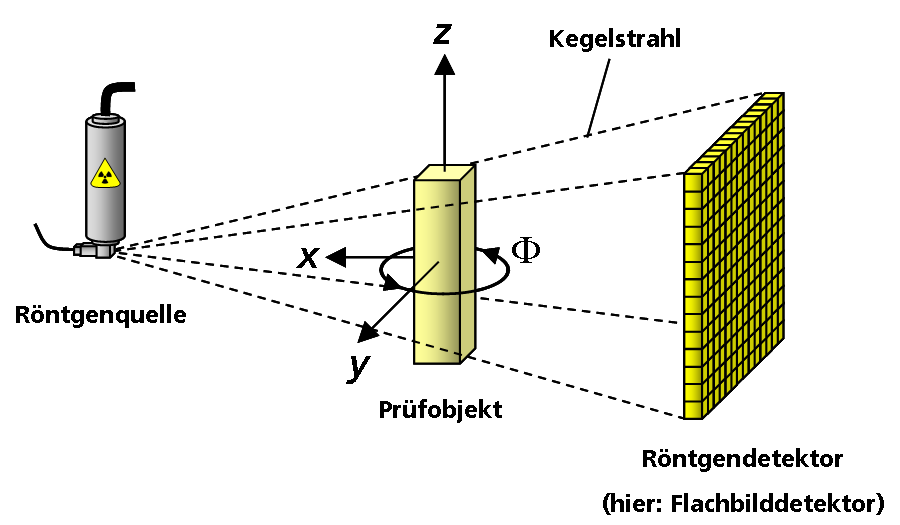
\includegraphics[height=0.618\textheight]{./images/3D_Computed_Tomography}
	\source{w.wiki/7g3}{\ccbysa}
\end{frame}

\begin{frame}{Examples}
	\centering
	\only<1|handout:1>{%
		\pgfmathsetlength{\imagewidth}{0.9\linewidth}%
		\pgfmathsetlength{\imagescale}{\imagewidth/3295}%
		\def\x{2036}% scalebar-x starting at golden ratio of image width of 3295px = 2036
		\def\y{1343}% scalebar-y at 90% of image height of 1492px = 1343
		\begin{tikzpicture}[x=\imagescale,y=-\imagescale]
			\node[anchor=north west, inner sep=0pt, outer sep=0pt] at (0,0) {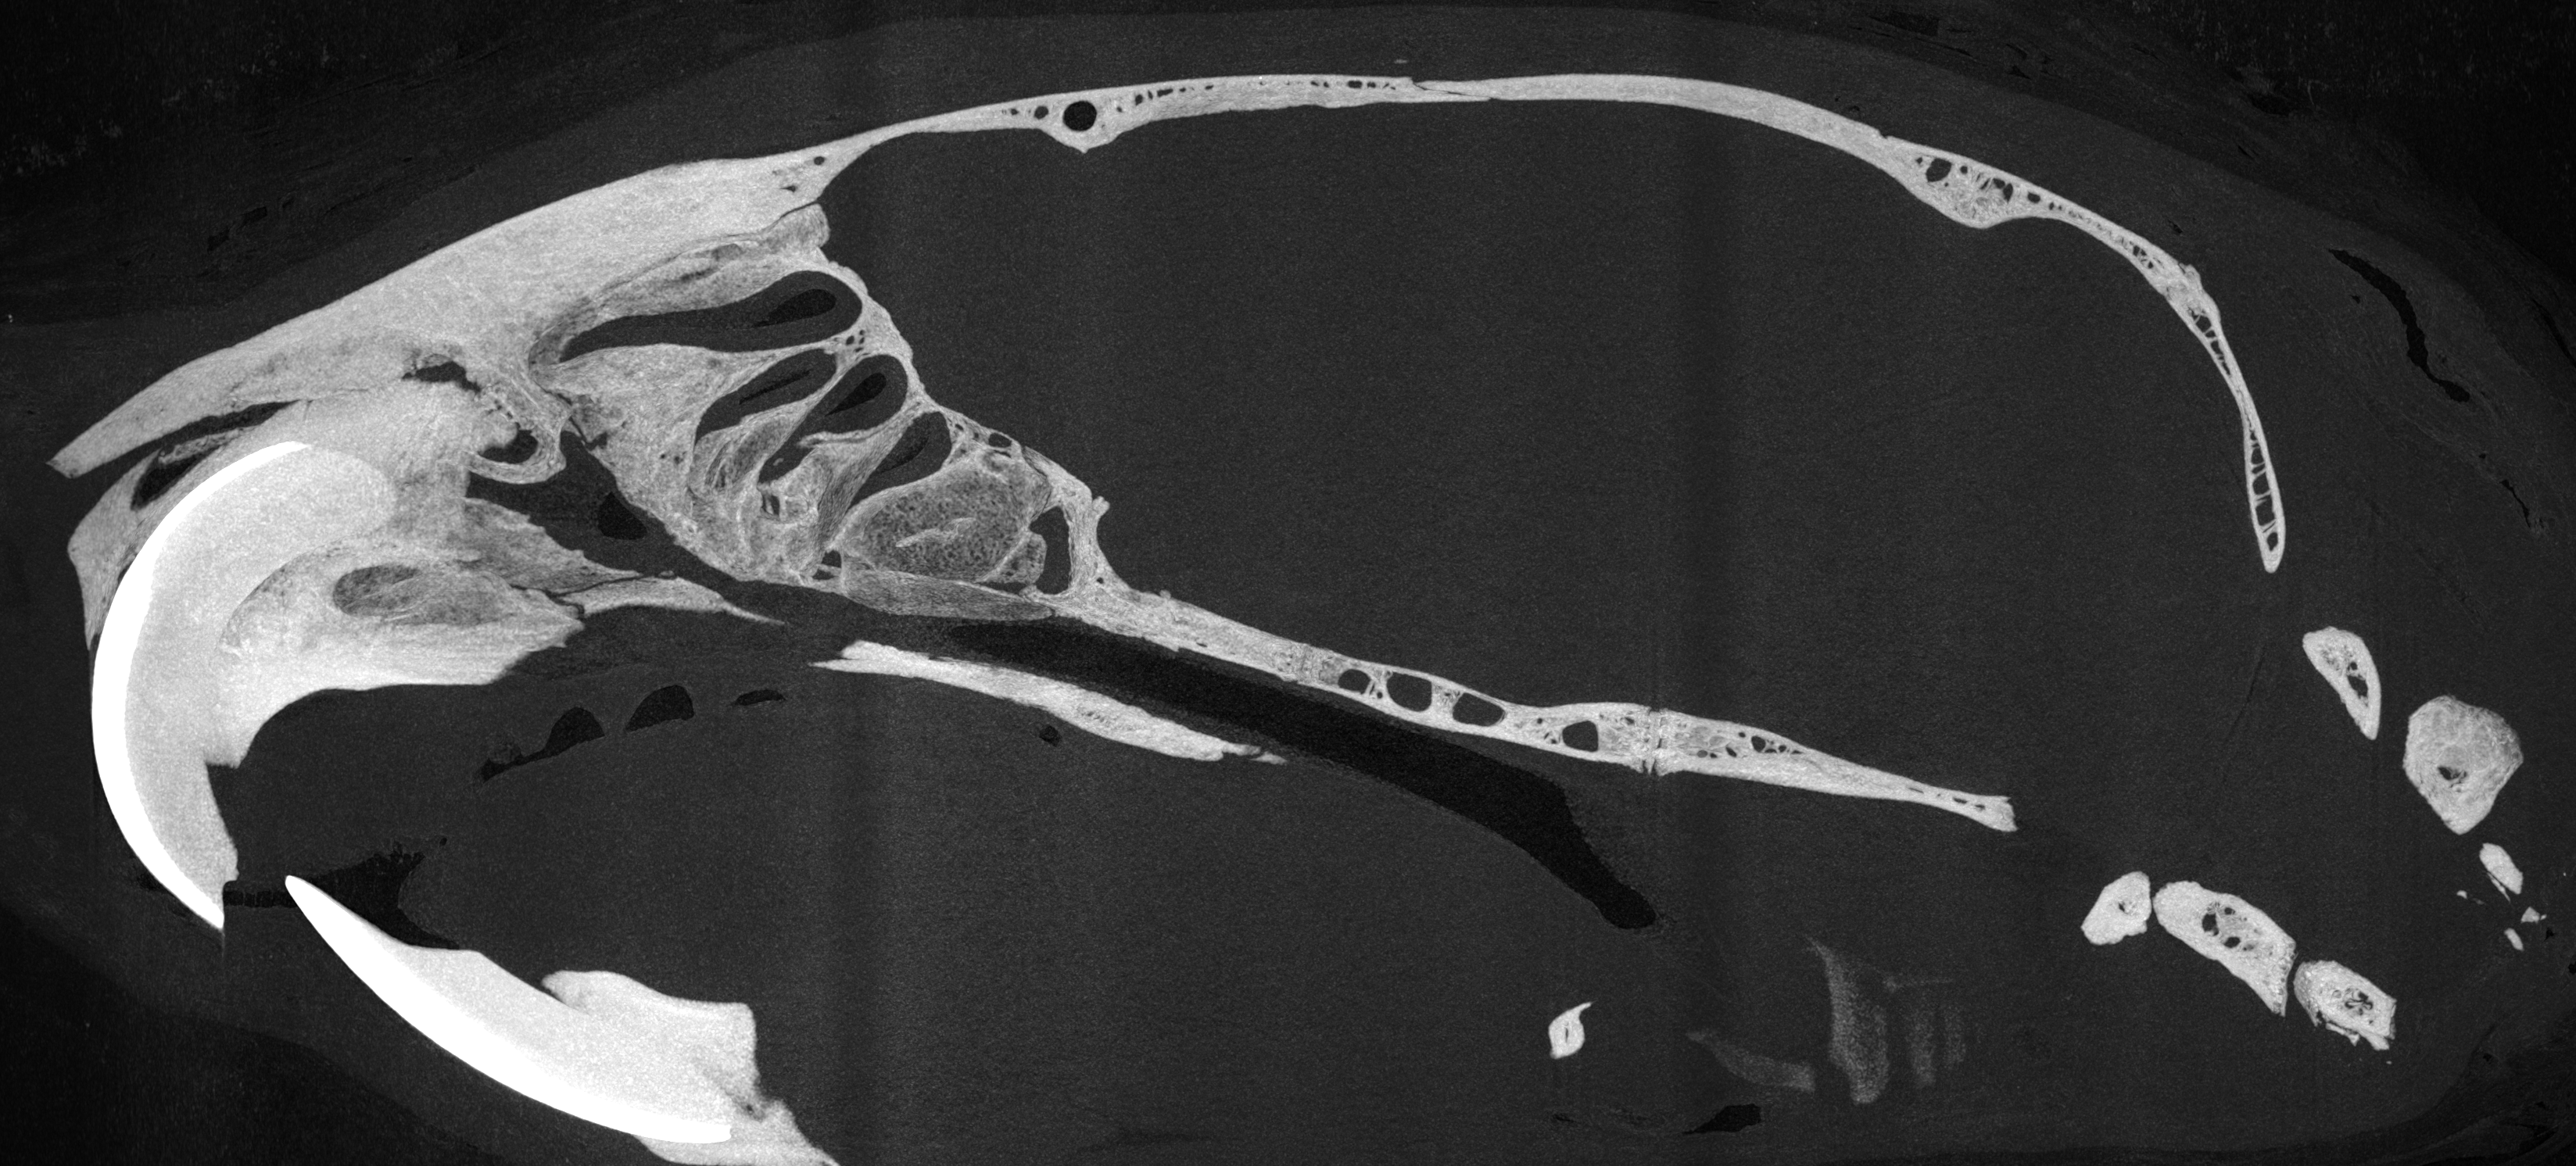
\includegraphics[width=\imagewidth]{./images/Mouse1265_resliced_MIP500um}};
			% 3295.000px = 26.2282mm -> 100px = 796.000um -> 62.814px = 500um, 12.563px = 100um
			%\draw[|-|,blue,thick] (0,746) -- (3295,746) node [sloped,midway,above,fill=white,semitransparent,text opacity=1] {\SI{26.2282}{\milli\meter} (3295px) TEMPORARY!};
			\draw[|-|,white,shadowed] (\x,\y) -- (\x+628.14,\y) node [midway,above] {\shadowtext{\SI{5}{\milli\meter}}};
		\end{tikzpicture}%
	}%
	\pgfmathsetlength{\imagewidth}{0.5\linewidth}%
	\pgfmathsetlength{\imagescale}{\imagewidth/2301}%
	\def\x{1422+450}% scalebar-x starting at golden ratio of image width of 2301px = 1422
	\def\y{1715}% scalebar-y at 90% of image height of 1906px = 1715
	\begin{tikzpicture}[x=\imagescale,y=-\imagescale]
		\only<2|handout:2>{%
			\node[anchor=north west, inner sep=0pt, outer sep=0pt] at (0,0) {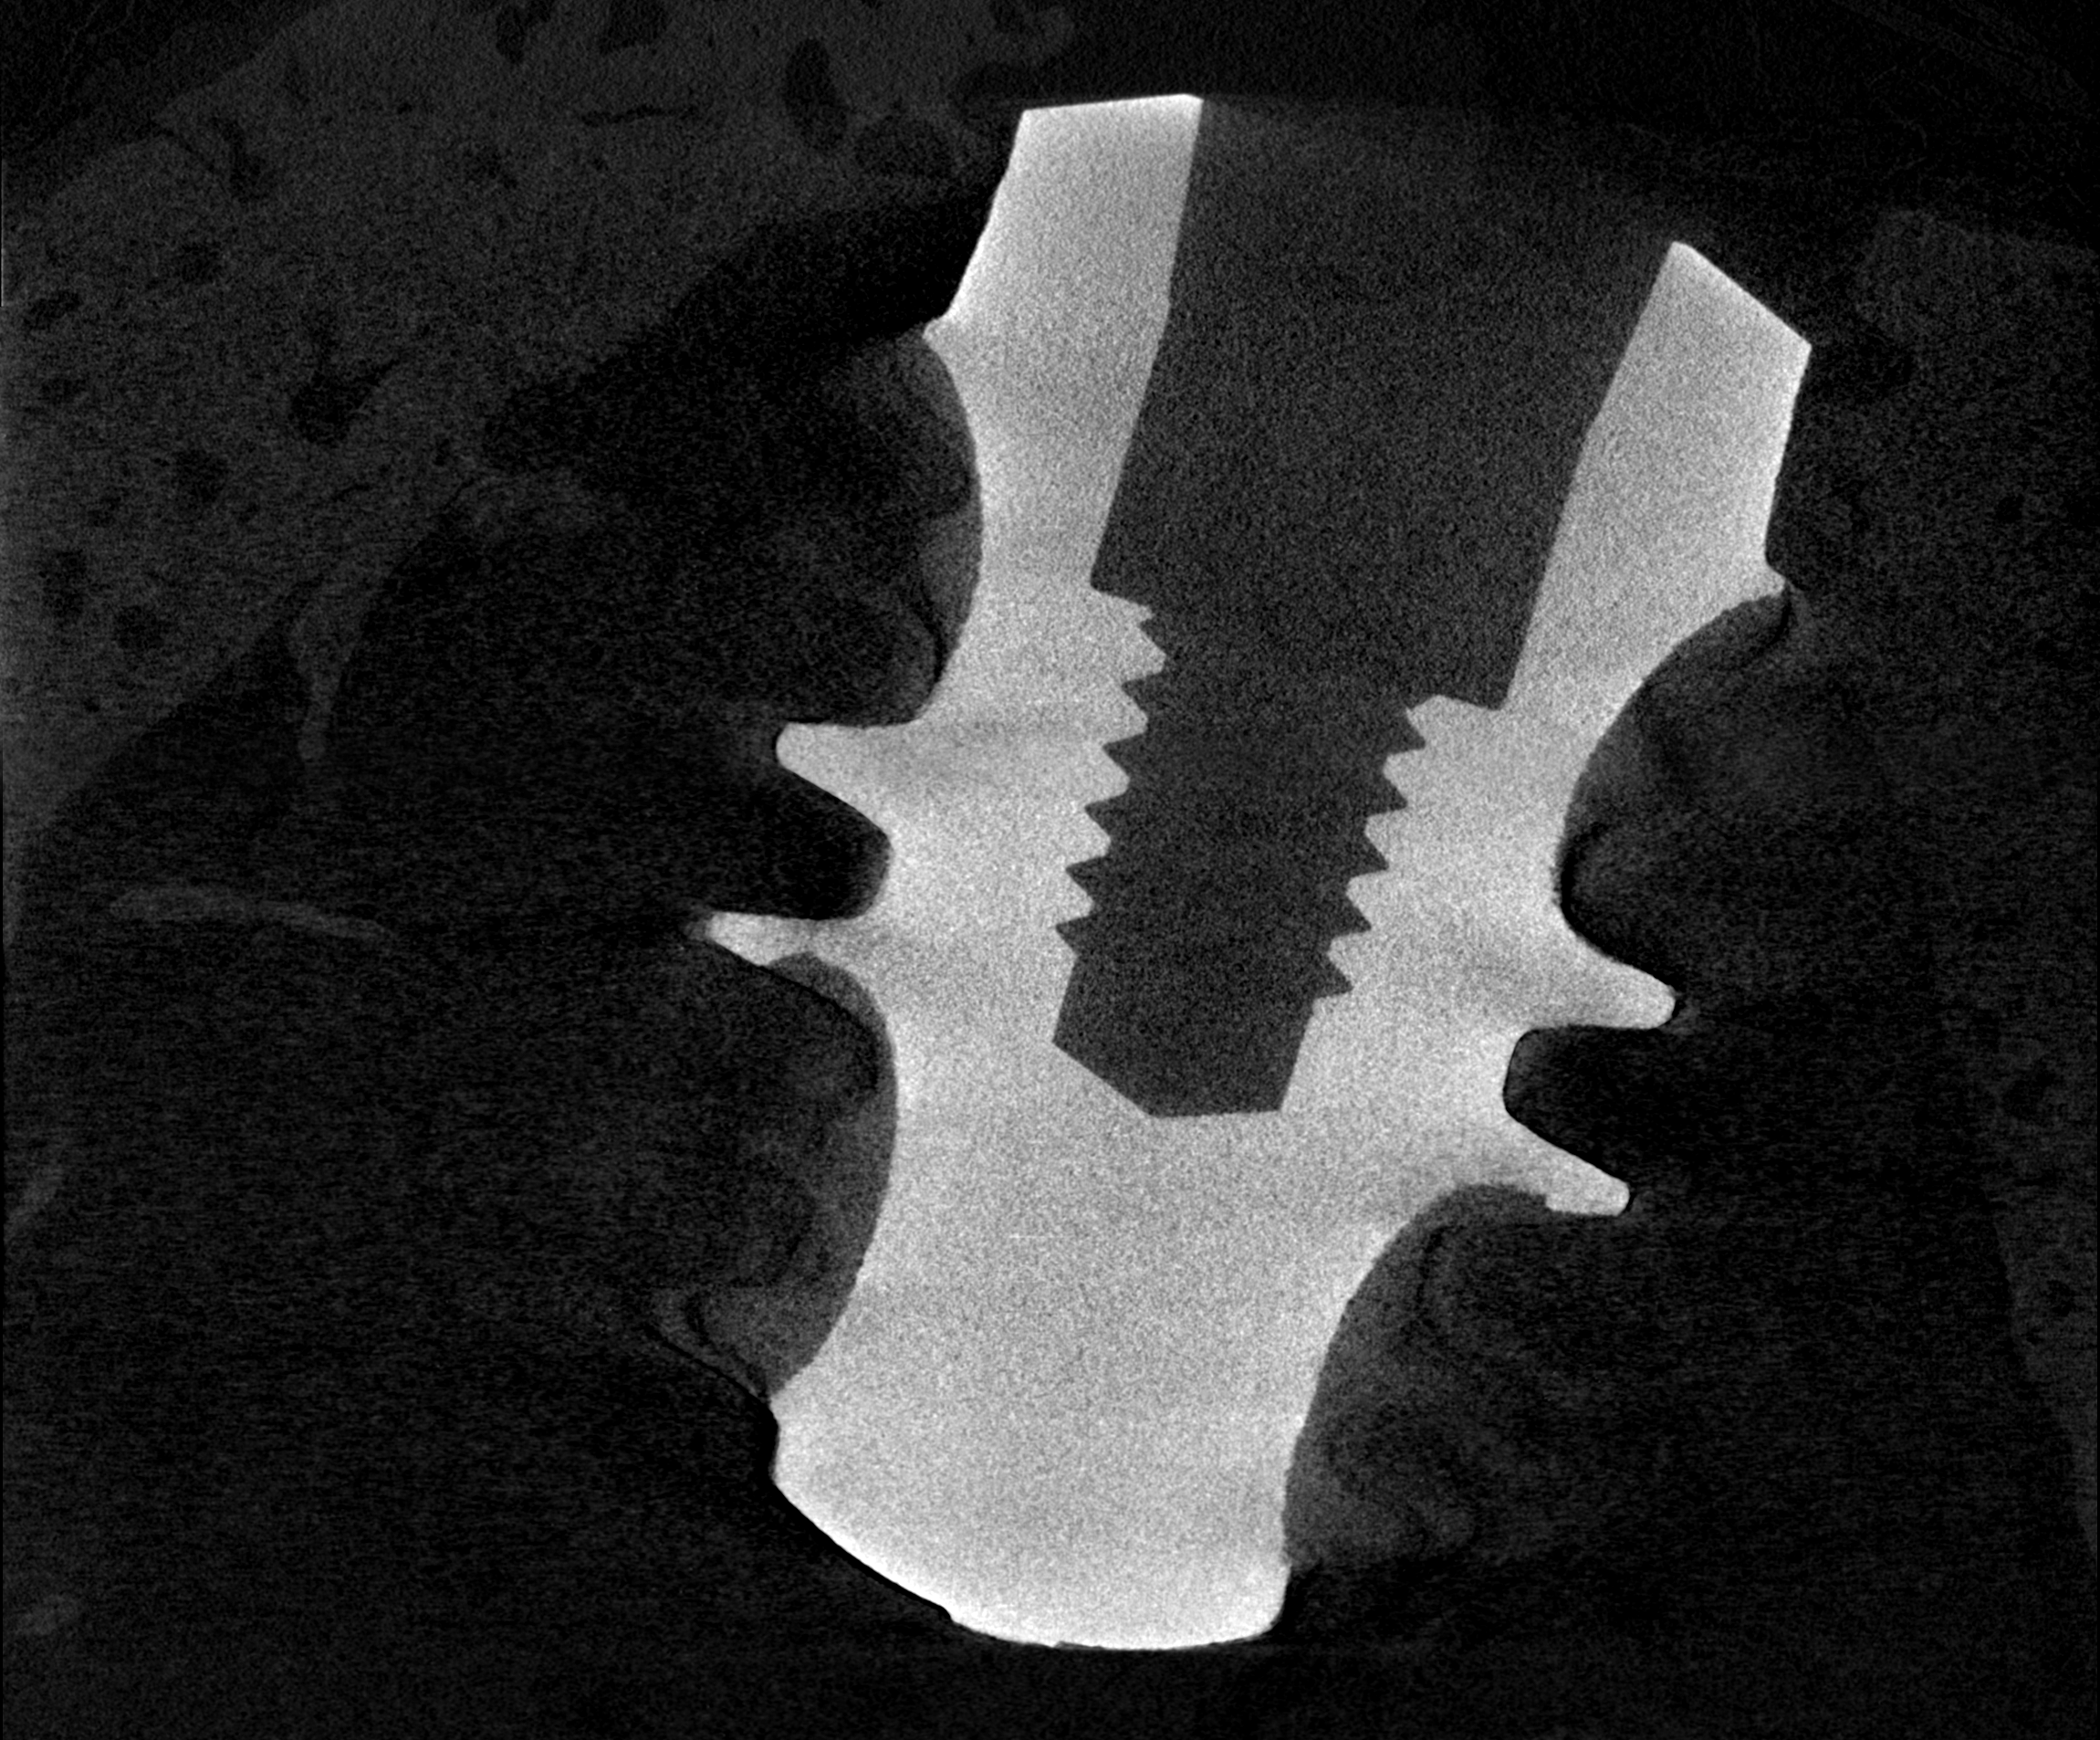
\includegraphics[width=\imagewidth]{./images/2834_left_post_Cu_011_1272_360_5um_reslice}};
		}%
		\only<3|handout:0>{%
			\node[anchor=north west, inner sep=0pt, outer sep=0pt] at (0,0) {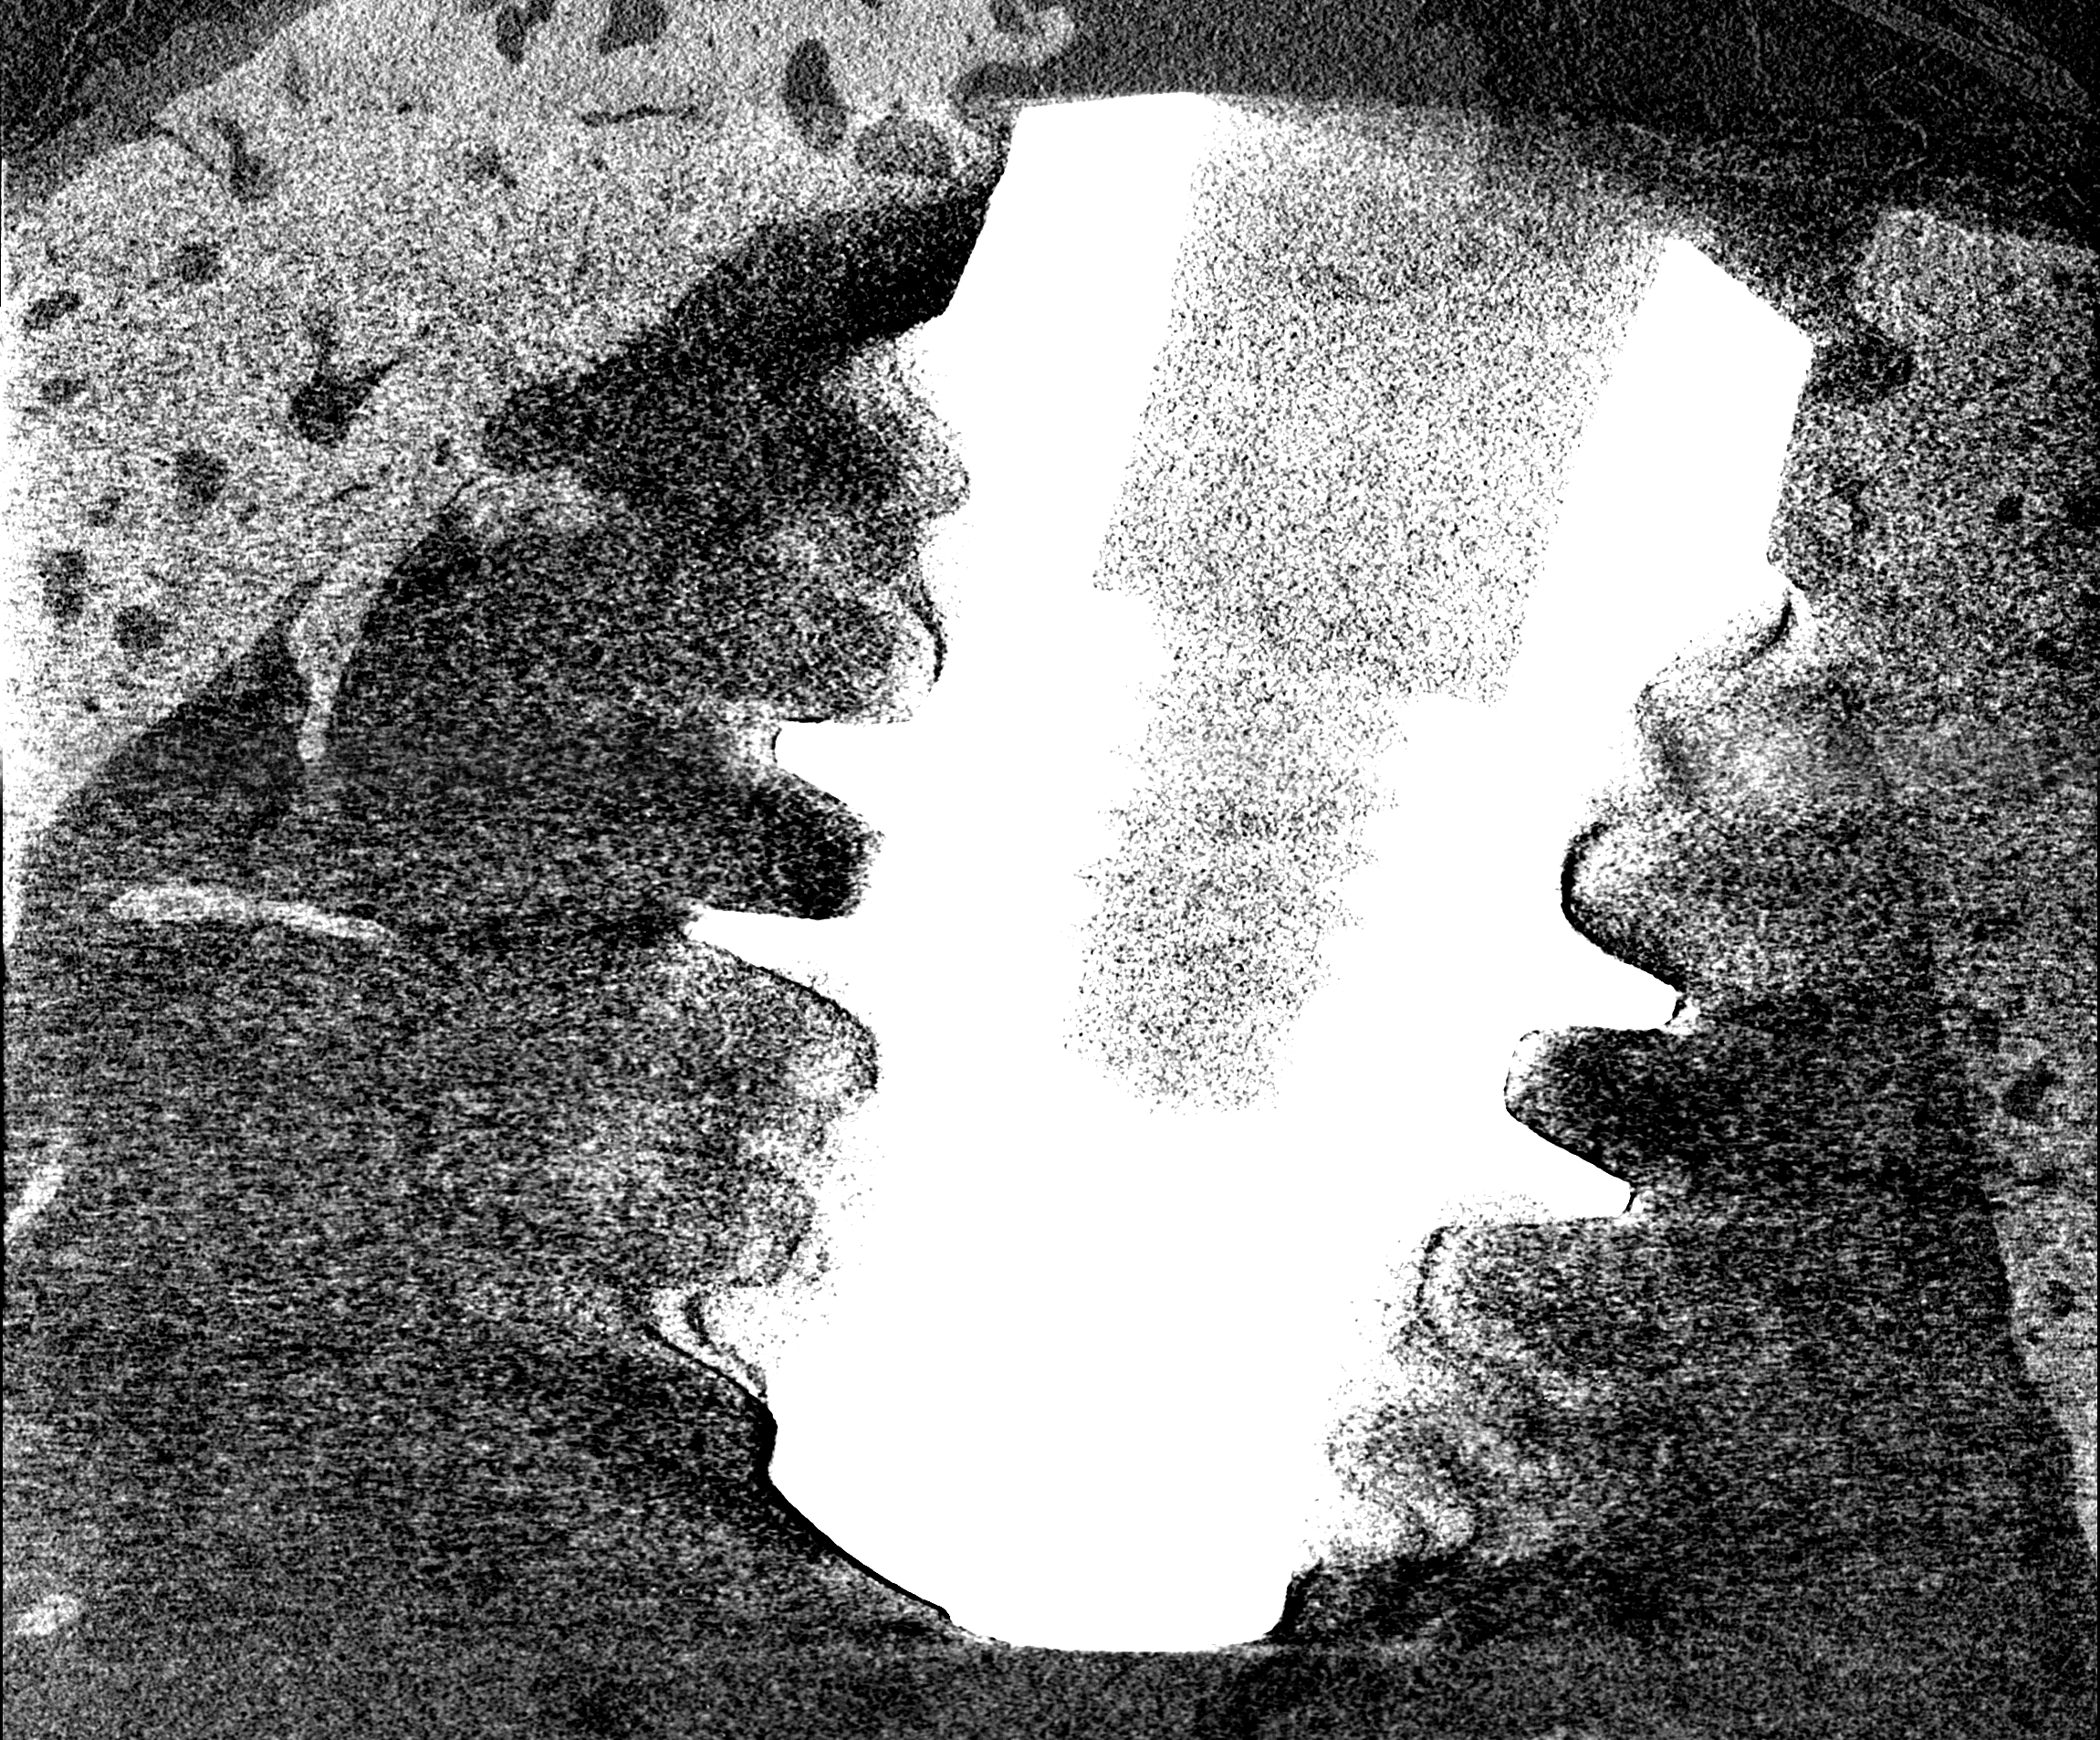
\includegraphics[width=\imagewidth]{./images/2834_left_post_Cu_011_1272_360_5um_reslice_stretched}};
		}%
		% 2301.000px = 11.505mm -> 100px = 500.000um -> 100.000px = 500um, 20.000px = 100um
		%\draw[|-|,blue,thick] (0,953) -- (2301,953) node [sloped,midway,above,fill=white,semitransparent,text opacity=1] {\SI{11.505}{\milli\meter} (2301px) TEMPORARY!};
		\only<2-3|handout:2>{%
			\draw[|-|,white,shadowed] (\x,\y) -- (\x+200,\y) node [midway,above] {\shadowtext{\SI{1}{\milli\meter}}};
		}
	\end{tikzpicture}%
	\only<4|handout:3>{%
		\pgfmathsetlength{\imagewidth}{0.618\linewidth}%
		\pgfmathsetlength{\imagescale}{\imagewidth/690}%
		\def\x{426}% scalebar-x starting at golden ratio of image width of 690px = 426
		\def\y{421}% scalebar-y at 90% of image height of 468px = 421
		\begin{tikzpicture}[x=\imagescale,y=-\imagescale]
			\node[anchor=north west, inner sep=0pt, outer sep=0pt] at (0,0) {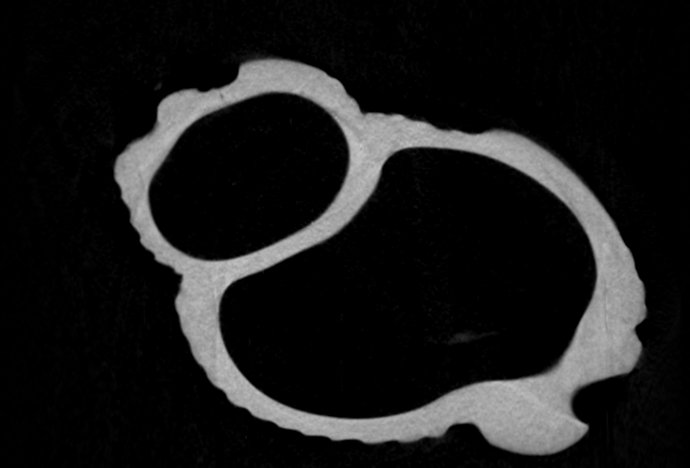
\includegraphics[width=\imagewidth]{./movies/shell/Muschel_klein0150}};
			% 690.000px = 7.452000000000001mm -> 100px = 1080.000um -> 46.296px = 500um, 9.259px = 100um
			%\draw[|-|,blue,thick] (0,234) -- (690,234) node [sloped,midway,above,fill=white,semitransparent,text opacity=1] {\SI{7.452000000000001}{\milli\meter} (690px) TEMPORARY!};
			\draw[|-|,white,shadowed] (\x,\y) -- (\x+92.59,\y) node [midway,above] {\shadowtext{\SI{1}{\milli\meter}}};
		\end{tikzpicture}%
	}
	\only<5|handout:0>{%
		\animategraphics[autoplay,loop,width=0.618\linewidth,every=\everyframe]{24}{./movies/shell/Muschel_klein}{0150}{431}
	}
	\only<6|handout:4>{%
		\pgfmathsetlength{\imagewidth}{0.42\linewidth}%
		\pgfmathsetlength{\imagescale}{\imagewidth/1224}%
		\def\x{756}% scalebar-x starting at golden ratio of image width of 1224px = 756
		\def\y{1102}% scalebar-y at 90% of image height of 1224px = 1102
		\begin{tikzpicture}[x=\imagescale,y=-\imagescale]
			\node[anchor=north west, inner sep=0pt, outer sep=0pt] at (0,0) {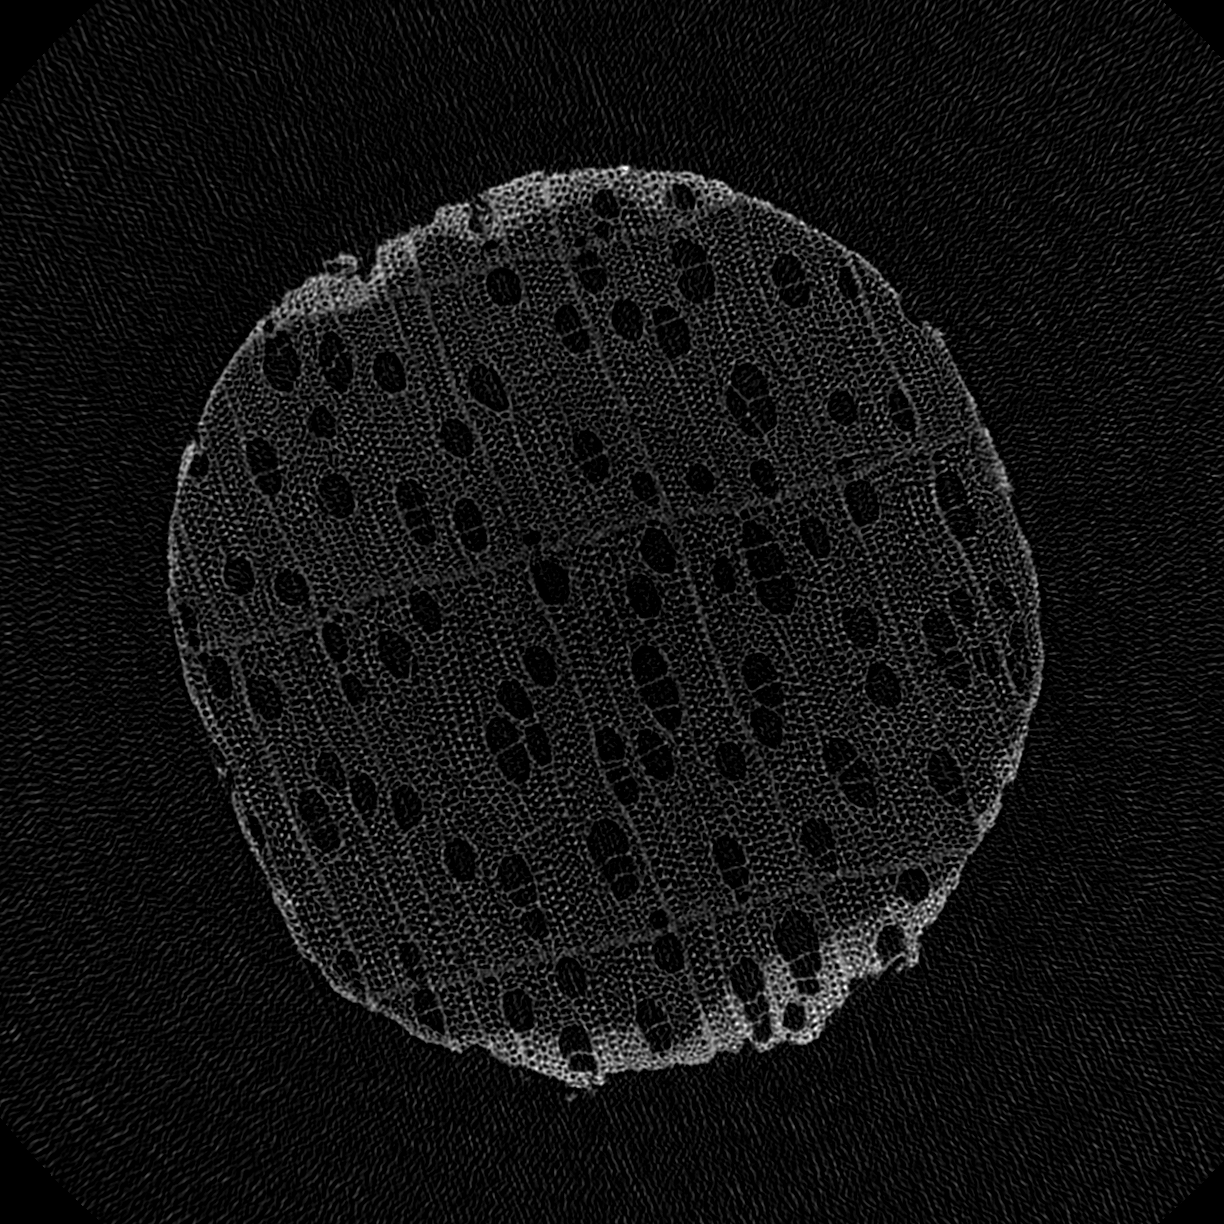
\includegraphics[width=\imagewidth]{./images/Toothpick_rec00000555}};
			% 1224.000px = 2.754mm -> 100px = 225.000um -> 222.222px = 500um, 44.444px = 100um
			%\draw[|-|,blue,thick] (0,612) -- (1224,612) node [sloped,midway,above,fill=white,semitransparent,text opacity=1] {\SI{2.754}{\milli\meter} (1224px) TEMPORARY!};
			\draw[|-|,white,shadowed] (\x,\y) -- (\x+222.222,\y) node [midway,above] {\shadowtext{\SI{500}{\micro\meter}}};
		\end{tikzpicture}%
	}
	\only<7|handout:5>{%
		\pgfmathsetlength{\imagewidth}{0.55\linewidth}%
		\pgfmathsetlength{\imagescale}{\imagewidth/708}%
		\def\x{438+150}% scalebar-x starting at golden ratio of image width of 708px = 438
		\def\y{463}% scalebar-y at 90% of image height of 514px = 463
		\begin{tikzpicture}[x=\imagescale,y=-\imagescale]
			\node[anchor=north west, inner sep=0pt, outer sep=0pt] at (0,0) {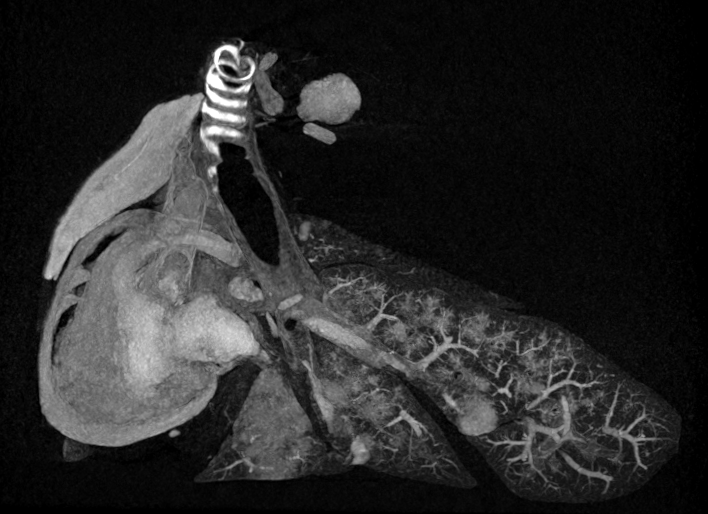
\includegraphics[width=\imagewidth]{./images/KP-TNIKWT2_rec_reslice_MIP500um}};
			% 708.000px = 15.292800000000002mm -> 100px = 2160.000um -> 23.148px = 500um, 4.630px = 100um
			%\draw[|-|,blue,thick] (0,257) -- (708,257) node [sloped,midway,above,fill=white,semitransparent,text opacity=1] {\SI{15.292800000000002}{\milli\meter} (708px) TEMPORARY!};
			\draw[|-|,white,shadowed] (\x,\y) -- (\x+46.3,\y) node [midway,above] {\shadowtext{\SI{1}{\milli\meter}}};
		\end{tikzpicture}%
	}
\end{frame}

\section{A scan, from \emph{getting started} to \emph{nice image}}
\begin{frame}{Preparation}
	\begin{itemize}
		\item Study design
		\item Sample preparation
	\end{itemize}
\end{frame}

\renewcommand{\imwidth}{0.49\linewidth}
\begin{frame}{Projections}
	\includegraphics[width=\imwidth]{./images/14_Physics_updated}%
	\sourcelink{ilias.unibe.ch/goto\_ilias3\_unibe\_sess\_1555733.html}{\emph{Laws of Physics for Microscopists} by Michael Jaeger}{Slide 14}%
	\hfill%
	\includegraphics[width=\imwidth]{./images/15_Physics_updated}%
	\sourcelink{ilias.unibe.ch/goto\_ilias3\_unibe\_sess\_1555733.html}{\emph{Laws of Physics for Microscopists} by Michael Jaeger}{Slide 15}%
\end{frame}

\begin{frame}{Projections}
	\centering
	% Movie frames generated with https://github.com/habi/Lecture.Microtomography/blob/master/Notebooks/FromProjectionsToReconstructions.ipynb
	\mode<beamer>{\animategraphics[autoplay,loop,height=\imheight,every=\everyframe]{24}{./movies/scan/projections/KP-TNIKWT02_240_projections_of_940_800_px_}{000}{313}}
	\mode<handout>{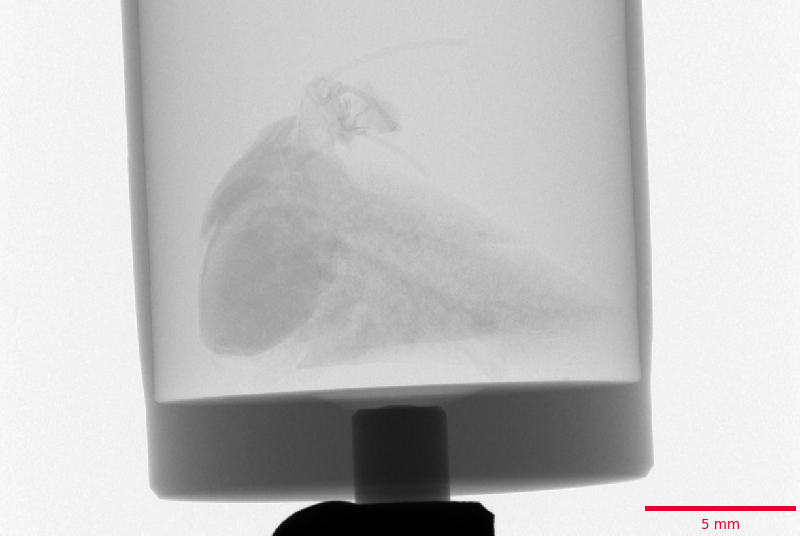
\includegraphics[height=\imheight]{./movies/scan/projections/KP-TNIKWT02_240_projections_of_940_800_px_000}}
\end{frame}

\begin{frame}{Projections}
	\begin{itemize}
		\item A (micro-focus) x-ray source illuminates the object
		\item The x-rays penetrate the sample and are attenuated
		\item A scintillator converts the x-rays to visible light
		\item A (planar) x-ray detector collects (magnified) projection images.
		\item The projections are recorded on disk
	\end{itemize}
\end{frame}

\begin{frame}{Reconstructions}
	\centering
	% Movie frames generated with https://github.com/habi/Lecture.Microtomography/blob/master/Notebooks/FromProjectionsToReconstructions.ipynb
	\mode<beamer>{\animategraphics[autoplay,palindrome,height=\imheight,every=\everyframe]{24}{./movies/scan/reconstructions/KP-TNIKWT02_240_reconstructions_of_556_800_px_}{000}{277}}
	\mode<handout>{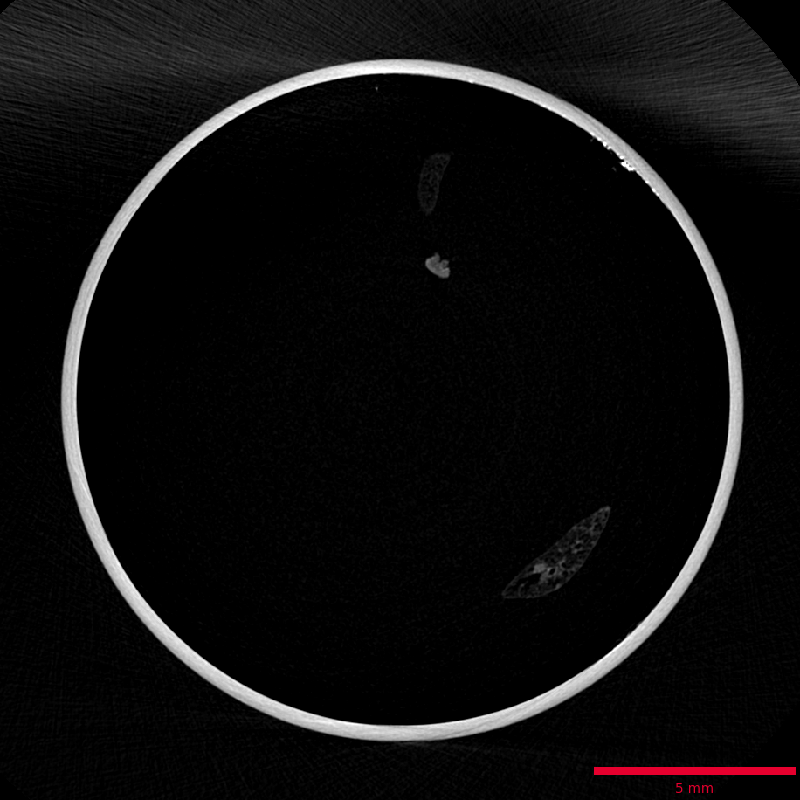
\includegraphics[height=\imheight]{./movies/scan/reconstructions/KP-TNIKWT02_240_reconstructions_of_556_800_px_000}}
\end{frame}

\begin{frame}{Reconstructions}
	\begin{itemize}
		\item Based on hundreds of angular views acquired while the object rotates, a computer synthesizes a stack of virtual cross section slices through the object.
		\item Radon Transformation
		\item Filtered back projection
		\item Fan beam reconstruction
		\item Corrections (beam hardening, etc.)
		\item Writing to stack
	\end{itemize}
\end{frame}

\begin{frame}{Visualization}
	\begin{tikzpicture}[remember picture,overlay]%
	\node at (current page.center){%
		\mode<beamer>{\animategraphics[autoplay,loop,height=\paperheight,every=\everyframe]{24}{./movies/scan/visualization/lung}{000}{240}}%
		\mode<handout>{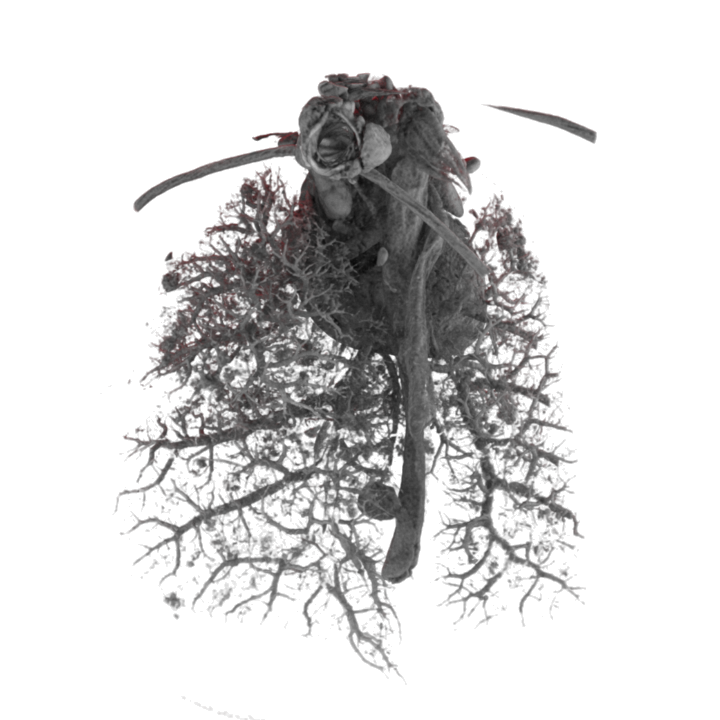
\includegraphics[height=\paperheight]{./movies/scan/visualization/lung000}}%
		};%
	\end{tikzpicture}%
\end{frame}

\begin{frame}{Visualization}
	\begin{itemize}
		\item Based the on reconstructions, a computer synthesizes a three-dimensional view of the scanned sample
	\end{itemize}
\end{frame}

\begin{frame}{What to use?}
	\begin{itemize}
		\item \href{http://fiji.sc/}{ImageJ/Fiji}~\cite{Schindelin2012}
		\item Also see \href{https://ilias.unibe.ch/goto_ilias3_unibe_sess_1561468.html}{\emph{Fundamentals of Digital Image Processing} by Guillaume Witz}
		\item Reproducible research
		\begin{itemize}
			\item \href{https://www.python.org/}{\faPython} in \href{https://jupyter.org/}{Jupyter}~\cite{Kluyver2016}
			\item \href{https://git-scm.com/}{\faGit}
			\item Script all your things!
			\item Data repositories; sharing is caring!
		\end{itemize}
	\end{itemize}
\end{frame}

\section{Example of a full study}
\begin{frame}{Quantitative data}
	\begin{itemize}
		\item Raw numbers instead of just pretty images
		\item Segmentation
		\item Characterization
	\end{itemize}
\end{frame}

\subsection{Overview}
\begin{frame}
	\frametitle{An example: Do gills change with training?}
	\centering
	% Image adapted from https://teacheratsea.files.wordpress.com/2011/07/gills-an-o2.jpg
	\includegraphics[height=\imheight]{./images/gills-and-o2}%
	\source{Campbell Biology}{\cite{Taylor2017}}
\end{frame}

\begin{frame}
	\frametitle{Gill anatomy}
	\begin{tikzpicture}[remember picture,overlay]%
		\node at (current page.center){%
			\mode<beamer>{\animategraphics[autoplay,width=\paperwidth,every=\everyframe]{24}{./movies/fishhead/head-without-gills0}{001}{160}}%
			\mode<handout>{\includegraphics[width=\paperwidth]{./movies/fishhead/head-without-gills0001}}%
			};%
	\end{tikzpicture}%
\end{frame}

\begin{frame}
	\frametitle{Gill anatomy}
	\begin{tikzpicture}[remember picture,overlay]%
\node at (current page.center){%
			\mode<beamer>{\animategraphics[autoplay,width=\paperwidth,every=\everyframe]{24}{./movies/fishhead/head-without-gills0}{161}{481}}%
			\mode<handout>{\includegraphics[width=\paperwidth]{./movies/fishhead/head-without-gills0333}}%
			};%
	\end{tikzpicture}%
\end{frame}

\subsection{Setup}
\renewcommand{\imwidth}{\columnwidth}
\begin{frame}{How?}
	\begin{columns}
		\begin{column}{0.49\linewidth}
			\begin{itemize}
				\item<1-> Training for \SI{5}{w}, \SI{5}{\day\per w}, \SI{6}{\hour\per\day}, at \SI{66}{\percent} of critical speed~\cite{Palstra2010}
				\begin{itemize}
					\item<1-> Endurance
				\end{itemize}
				\item<3-|handout:2-> Morphology \& Physiology
				\begin{itemize}
					\item<3-|handout:2-> Body size \& weight
					\item<3-|handout:2-> \ce{O2} consumption
				\end{itemize}
				\item<4-|handout:3-> Scanning electron microscopy
				\begin{itemize}
					\item<4-|handout:3-> Gill structure
				\end{itemize}
				\item<5-|handout:4-> Critical point drying\onslide<6-|handout:5->{, \uct imaging}\onslide<7-|handout:6->{, delineation in CTAn }\onslide<8-|handout:7->{and analysis}
				\begin{itemize}
					\item<8-|handout:7-> Gill volume, structure and complexity
				\end{itemize}
			\end{itemize}
		\end{column}
		\begin{column}{0.49\linewidth}
			\only<1|handout:1>{%
				\pgfmathsetlength{\imagewidth}{\imwidth}%
				\pgfmathsetlength{\imagescale}{\imagewidth/1080}%
				\def\x{667}% scalebar-x starting at golden ratio of image width of 1080px = 667
				\def\y{547}% scalebar-y at 90% of image height of 608px = 547
				\begin{tikzpicture}[x=\imagescale,y=-\imagescale]%
					\node[anchor=north west, inner sep=0pt, outer sep=0pt] at (0,0) {\includegraphics[width=\imwidth]{./movies/training/fishvideo_0001}};%
					% 69px = 30mm > 100px = 44mm > 1142px = 500mm, 228px = 100mm
					%\draw[|-|,blue] (410,188) -- (478,182) node [sloped,midway,above,fill=white,semitransparent,text opacity=1] {\SI{30}{\milli\meter} (TEMPORARY)};
					\draw[|-|,white] (\x,\y) -- (\x+228.4,\y) node [midway,above] {\(\approx\)\SI{10}{\centi\meter}};%
				\end{tikzpicture}%
				}%
			\only<2|handout:0>{%
				\animategraphics[loop,autoplay,width=\linewidth,every=\everyframe]{24}{./movies/training/fishvideo_0}{001}{250}%
				}%
			\only<3|handout:2>{\centering\Huge\faFish:\xspace\faRuler\xspace\&\xspace\faWeight}
			\renewcommand{\imwidth}{0.49\columnwidth}%
			\only<4|handout:3>{%
				\pgfmathsetlength{\imagewidth}{\imwidth}%
				\pgfmathsetlength{\imagescale}{\imagewidth/794}%
				\def\x{491}% scalebar-x starting at golden ratio of image width of 794px = 491
				\def\y{458}% scalebar-y at 90% of image height of 509px = 458
				\begin{tikzpicture}[x=\imagescale,y=-\imagescale]%
					\node[anchor=north west, inner sep=0pt, outer sep=0pt] at (0,0) {\includegraphics[width=\imwidth]{./images/EM_c5_3}};%
					% 794px = 2.4111398mm > 100px = 304um > 165px = 500um, 33px = 100um
					%\draw[|-|,blue] (0,298) -- (794,298) node [sloped,midway,above,fill=white,semitransparent,text opacity=1] {\SI{2.4111398}{\milli\meter} (794px) TEMPORARY!};
					\draw[|-|,white,shadowed] (\x,\y) -- (\x+165,\y) node [midway,above] {\shadowtext{\SI{500}{\micro\meter}}};%
				\end{tikzpicture}%
				\begin{tikzpicture}[x=\imagescale,y=-\imagescale]%
					\node[anchor=north west, inner sep=0pt, outer sep=0pt] at (0,0) {\includegraphics[width=\imwidth]{./images/EM_s5_3}};%
					% 794px = 2.4111398mm > 100px = 304um > 165px = 500um, 33px = 100um
					%\draw[|-|,blue] (0,298) -- (794,298) node [sloped,midway,above,fill=white,semitransparent,text opacity=1] {\SI{2.4111398}{\milli\meter} (794px) TEMPORARY!};
					\draw[|-|,white,shadowed] (\x,\y) -- (\x+165,\y) node [midway,above] {\shadowtext{\SI{500}{\micro\meter}}};%
				\end{tikzpicture}%
				}
			\renewcommand{\imwidth}{\columnwidth}
			\only<5|handout:4>{%
				\centering
				\pgfmathsetlength{\imagewidth}{\imwidth}%
				\pgfmathsetlength{\imagescale}{\imagewidth/1080}%
				\def\x{667}% scalebar-x starting at golden ratio of image width of 1080px = 667
				\def\y{673}% scalebar-y at 90% of image height of 748px = 673
				\begin{tikzpicture}[x=\imagescale,y=-\imagescale]
					\node[anchor=north west, inner sep=0pt, outer sep=0pt] at (0,0) {\includegraphics[width=\imwidth]{./images/IMG_20190603_174659}};
					% 294px = 12.5mm > 100px = 4250um > 118px = 5mm
					%\draw[|-|,blue,thick] (494,218) -- (624,481) node [sloped,midway,above,fill=white,semitransparent,text opacity=1] {\SI{12.5}{\milli\meter} (294px) TEMPORARY!};
					\draw[|-|,white,shadowed] (\x,\y) -- (\x+118,\y) node [midway,above] {\shadowtext{\SI{5}{\milli\meter}}};
				\end{tikzpicture}%
				}
			\only<6|handout:5>{%
				\lstinputlisting[linerange={2-5,17-17,19-23,29-31,34-34,38-40,51-51,58-59}]{./logfiles/Control05/proj/Control05.log}%
				}
			\includegraphics<7|handout:6>[height=\imheight]{./images/CTAn}%
			\only<8|handout:7>{%
				\mode<beamer>{%
					\animategraphics[loop,autoplay,width=\linewidth,every=\everyframe]{24}{./movies/coder/coder-}{0}{133}%
					\source{gph.is/2nqkple}{}%
					}%
				\mode<handout>{%
					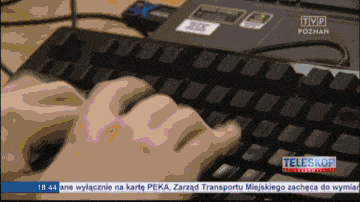
\includegraphics[width=\linewidth]{./movies/coder/coder-0}
					\source{gph.is/2nqkple}{}%
					}%
				}
		\end{column}
	\end{columns}
\end{frame}
\note{Comparable with the weekly training routine of Michael Phelps.
	The fish trained only for ca. \SI{7}{\percent} of their lifetime and started as adults.
	The Olympic winner trained for half of his lifetime and started as child.}
\note{We analyzed 20 samples with a mean size of a cube with a side length of 1863 pixels.
	This means we analyzed 129.40 Gigapixels.
	This means we analyzed \num{129395.29} Megapixels.
	In total \num{46014} slices.}
	


\subsection{Image processing}
\begin{frame}
	\frametitle{Gill volume}
	\centering
	\only<1|handout:1>{%
		\pgfmathsetlength{\imagewidth}{0.4\linewidth}%
		\pgfmathsetlength{\imagescale}{\imagewidth/2524}%
		\def\x{1560}% scalebar-x starting at golden ratio of image width of 2524px = 1560
		\def\y{2272}% scalebar-y at 90% of image height of 2524px = 2272
		\begin{tikzpicture}[x=\imagescale,y=-\imagescale]
			\node[anchor=north west, inner sep=0pt, outer sep=0pt] at (0,0) {\includegraphics[width=\imagewidth]{./images/Control03_rec00001865}};
			% 2524px = 4.1874422mm > 100px = 166um > 301px = 500um, 60px = 100um
			%\draw[|-|,blue] (0,1262) -- (2524,1262) node [sloped,midway,above,fill=white,semitransparent,text opacity=1] {\SI{4.18}{\milli\meter} (2524px) TEMPORARY!};
			\draw[|-|,white,shadowed] (\x,\y) -- (\x+301,\y) node [midway,above] {\shadowtext{\SI{500}{\micro\meter}}};
		\end{tikzpicture}%
	}%
	\pgfmathsetlength{\imagewidth}{0.618\linewidth}%
	\pgfmathsetlength{\imagescale}{\imagewidth/2163}%
	\def\x{1730}% scalebar-x starting at golden ratio of image width of 2163px = 1337
	\def\y{1191}% scalebar-y at 90% of image height of 1323px = 1191
	\only<2|handout:2>{%
		\begin{tikzpicture}[x=\imagescale,y=-\imagescale]
			\node[anchor=north west, inner sep=0pt, outer sep=0pt] at (0,0) {\includegraphics[width=\imagewidth]{./images/Control03_rec00001865_crop}};
			% 2163px = 3.5885251499999997mm > 100px = 166um > 301px = 500um, 60px = 100um
			\draw[|-|,white,shadowed] (\x,\y) -- (\x+301,\y) node [midway,above] {\shadowtext{\SI{500}{\micro\meter}}};
		\end{tikzpicture}%
		}%
	\only<3|handout:3>{%
		\begin{tikzpicture}[x=\imagescale,y=-\imagescale]
			\node[anchor=north west, inner sep=0pt, outer sep=0pt] at (0,0) {\includegraphics[width=\imagewidth]{./images/Control03_rec0000_voi_1865_crop}};
			\draw[|-|,white,shadowed] (\x,\y) -- (\x+301,\y) node [midway,above] {\shadowtext{\SI{500}{\micro\meter}}};
		\end{tikzpicture}%
		}%
	\only<4|handout:4>{%
		\begin{tikzpicture}[x=\imagescale,y=-\imagescale]
			\node[anchor=north west, inner sep=0pt, outer sep=0pt] at (0,0) {\includegraphics[width=\imagewidth]{./images/Control03_thresholded_1500_crop}};
			\draw[|-|,white,shadowed] (\x,\y) -- (\x+301,\y) node [midway,above] {\shadowtext{\SI{500}{\micro\meter}}};
		\end{tikzpicture}%
		}%
	\only<5|handout:5>{\include{./plots/Gillvolume}}
	\only<6|handout:0>{\include{./plots/Gillvolume_scaled}}
\end{frame}

\begin{frame}{Gill complexity}
	\centering
	\pgfmathsetlength{\imagewidth}{0.618\linewidth}%
	\pgfmathsetlength{\imagescale}{\imagewidth/2163}%
	\def\x{1730}% scalebar-x starting at golden ratio of image width of 2163px = 1337
	\def\y{1191}% scalebar-y at 90% of image height of 1323px = 1191
	\only<1|handout:1>{%
		\begin{tikzpicture}[x=\imagescale,y=-\imagescale]
			\node[anchor=north west, inner sep=0pt, outer sep=0pt] at (0,0) {\includegraphics[width=\imagewidth]{./images/Control03_thresholded_1500_crop}};
			\draw[|-|,white,shadowed] (\x,\y) -- (\x+301,\y) node [midway,above] {\shadowtext{\SI{500}{\micro\meter}}};
		\end{tikzpicture}%
		}%
	\only<2|handout:2>{%
		\begin{tikzpicture}[x=\imagescale,y=-\imagescale]
			\node[anchor=north west, inner sep=0pt, outer sep=0pt] at (0,0) {\includegraphics[width=\imagewidth]{./images/Control03_area_organ_1500_crop_edit}};
			\draw[|-|,white,shadowed] (\x,\y) -- (\x+301,\y) node [midway,above] {\shadowtext{\SI{500}{\micro\meter}}};
		\end{tikzpicture}%
		}%
	\only<3|handout:3>{%
		\begin{tikzpicture}[x=\imagescale,y=-\imagescale]
			\node[anchor=north west, inner sep=0pt, outer sep=0pt] at (0,0) {\includegraphics[width=\imagewidth]{./images/Control03_area_organ_1500_crop_combination}};
			\draw[|-|,white,shadowed] (\x,\y) -- (\x+301,\y) node [midway,above] {\shadowtext{\SI{500}{\micro\meter}}};
		\end{tikzpicture}%
		}%
	\only<4|handout:4>{%
		\begin{tikzpicture}[remember picture,overlay]%
			\node at (current page.center){%
				\mode<beamer>{\animategraphics[palindrome,autoplay,width=\paperwidth,every=\everyframe]{24}{./movies/complexity/control03_thresholded_0}{030}{256}}%
				\mode<handout>{\includegraphics[width=\paperwidth]{./movies/complexity/control03_thresholded_0068}}%
				};%
		\end{tikzpicture}%
		}%
	\only<5|handout:5>{\include{./plots/Gills_per_organ}}
	\only<6|handout:0>{\include{./plots/Gills_per_organ_scaled}}
\end{frame}

\begin{frame}{Thanks!}
	\begin{itemize}
		\item Thanks for listening to me!
		\item<2-> \href{https://twitter.com/jackiantonovich/status/1195699076056178691}{What questions do you have for me?}
	\end{itemize}
	\only<3|handout:0>{%
		\begin{tikzpicture}[remember picture,overlay]%
			\node at (current page.center){%
				\animategraphics[loop,autoplay,width=\paperwidth,every=\everyframe]{24}{./movies/mouse_skull/mouse_skull}{000}{236}%
				};%
		\end{tikzpicture}%
	}%
\end{frame}

\begin{frame}{\href{https://en.wikipedia.org/wiki/Colophon_(publishing)}{Colophon}}
	\begin{itemize}
		\item This \textsc{beamer} presentation was crafted in \LaTeX\xspace with the (slightly adapted) \href{http://intern.unibe.ch/dienstleistungen/corporate_design_und_vorlagen/praesentationen/index_ger.html}{template from \emph{Corporate Design und Vorlagen} of the University of Bern}.
		\begin{itemize}
			\item \href{https://github.com/habi/lecture.microtomography/}{Complete source code: git.io/fjpP7}
			\item The \LaTeX\xspace code is automatically compiled with a \href{https://github.com/actions}{GitHub action}\footnote{Details on how this works are specified in a \href{https://github.com/habi/latex-test/}{small test repository here: git.io/JeOOj}} to a \href{https://habi.github.io/Lecture.Microtomography/XRayMicroTomography.Handout.pdf}{(handout) PDF which you can access here: git.io/JeQxO}
		\end{itemize}
		\item Did you spot an error?
		\begin{itemize}
			\item \href{https://github.com/habi/lecture.microtomography/issues}{File an issue: git.io/fjpPb}
			\item \href{https://github.com/habi/lecture.microtomography/pulls}{Submit a pull request: git.io/fjpPN}
			\item \href{mailto:haberthuer@ana.unibe.ch?subject=Error\%20in\%20the\%20(micro)-tomography\%20lecture\&body=https://xkcd.com/386/}{Send me an email: haberthuer@ana.unibe.ch}
		\end{itemize}
	\end{itemize}
\end{frame}

\begin{frame}{References}
	% Make the references continuously smaller :)
	%\renewcommand*{\bibfont}{\small}
	%\renewcommand*{\bibfont}{\footnotesize}
	%\renewcommand*{\bibfont}{\scriptsize}
	\renewcommand*{\bibfont}{\tiny}
	\setbeamertemplate{bibliography item}{\insertbiblabel}
	\printbibliography
\end{frame}

\end{document}
